% Options for packages loaded elsewhere
\PassOptionsToPackage{unicode}{hyperref}
\PassOptionsToPackage{hyphens}{url}
\PassOptionsToPackage{dvipsnames,svgnames,x11names}{xcolor}
%
\documentclass[
  12pt,
  12pt]{article}

\usepackage{amsmath,amssymb}
\usepackage{setspace}
\usepackage{iftex}
\ifPDFTeX
  \usepackage[T1]{fontenc}
  \usepackage[utf8]{inputenc}
  \usepackage{textcomp} % provide euro and other symbols
\else % if luatex or xetex
  \usepackage{unicode-math}
  \defaultfontfeatures{Scale=MatchLowercase}
  \defaultfontfeatures[\rmfamily]{Ligatures=TeX,Scale=1}
\fi
\usepackage{lmodern}
\ifPDFTeX\else  
    % xetex/luatex font selection
\fi
% Use upquote if available, for straight quotes in verbatim environments
\IfFileExists{upquote.sty}{\usepackage{upquote}}{}
\IfFileExists{microtype.sty}{% use microtype if available
  \usepackage[]{microtype}
  \UseMicrotypeSet[protrusion]{basicmath} % disable protrusion for tt fonts
}{}
\makeatletter
\@ifundefined{KOMAClassName}{% if non-KOMA class
  \IfFileExists{parskip.sty}{%
    \usepackage{parskip}
  }{% else
    \setlength{\parindent}{0pt}
    \setlength{\parskip}{6pt plus 2pt minus 1pt}}
}{% if KOMA class
  \KOMAoptions{parskip=half}}
\makeatother
\usepackage{xcolor}
\setlength{\emergencystretch}{3em} % prevent overfull lines
\setcounter{secnumdepth}{5}
% Make \paragraph and \subparagraph free-standing
\ifx\paragraph\undefined\else
  \let\oldparagraph\paragraph
  \renewcommand{\paragraph}[1]{\oldparagraph{#1}\mbox{}}
\fi
\ifx\subparagraph\undefined\else
  \let\oldsubparagraph\subparagraph
  \renewcommand{\subparagraph}[1]{\oldsubparagraph{#1}\mbox{}}
\fi


\providecommand{\tightlist}{%
  \setlength{\itemsep}{0pt}\setlength{\parskip}{0pt}}\usepackage{longtable,booktabs,array}
\usepackage{calc} % for calculating minipage widths
% Correct order of tables after \paragraph or \subparagraph
\usepackage{etoolbox}
\makeatletter
\patchcmd\longtable{\par}{\if@noskipsec\mbox{}\fi\par}{}{}
\makeatother
% Allow footnotes in longtable head/foot
\IfFileExists{footnotehyper.sty}{\usepackage{footnotehyper}}{\usepackage{footnote}}
\makesavenoteenv{longtable}
\usepackage{graphicx}
\makeatletter
\def\maxwidth{\ifdim\Gin@nat@width>\linewidth\linewidth\else\Gin@nat@width\fi}
\def\maxheight{\ifdim\Gin@nat@height>\textheight\textheight\else\Gin@nat@height\fi}
\makeatother
% Scale images if necessary, so that they will not overflow the page
% margins by default, and it is still possible to overwrite the defaults
% using explicit options in \includegraphics[width, height, ...]{}
\setkeys{Gin}{width=\maxwidth,height=\maxheight,keepaspectratio}
% Set default figure placement to htbp
\makeatletter
\def\fps@figure{htbp}
\makeatother

\addtolength{\oddsidemargin}{-.5in}%
\addtolength{\evensidemargin}{-1in}%
\addtolength{\textwidth}{1in}%
\addtolength{\textheight}{1.7in}%
\addtolength{\topmargin}{-1in}%
\usepackage{amsmath}
\numberwithin{equation}{section}
\usepackage{float}
\floatplacement{figure}{H}
\usepackage{threeparttable}
\usepackage{dcolumn}
\newcolumntype{d}[1]{D{.}{.}{#1}}
\usepackage{setspace}\onehalfspacing
\usepackage{multirow}
\usepackage{dsfont}
\usepackage{caption}
\captionsetup[table]{skip=5pt}
\usepackage{lscape}
\renewcommand{\arraystretch}{1.3}
\newcommand{\blandscape}{\begin{landscape}}
\newcommand{\elandscape}{\end{landscape}}
\makeatletter
\@ifpackageloaded{caption}{}{\usepackage{caption}}
\AtBeginDocument{%
\ifdefined\contentsname
  \renewcommand*\contentsname{Table of contents}
\else
  \newcommand\contentsname{Table of contents}
\fi
\ifdefined\listfigurename
  \renewcommand*\listfigurename{List of Figures}
\else
  \newcommand\listfigurename{List of Figures}
\fi
\ifdefined\listtablename
  \renewcommand*\listtablename{List of Tables}
\else
  \newcommand\listtablename{List of Tables}
\fi
\ifdefined\figurename
  \renewcommand*\figurename{Figure}
\else
  \newcommand\figurename{Figure}
\fi
\ifdefined\tablename
  \renewcommand*\tablename{Table}
\else
  \newcommand\tablename{Table}
\fi
}
\@ifpackageloaded{float}{}{\usepackage{float}}
\floatstyle{ruled}
\@ifundefined{c@chapter}{\newfloat{codelisting}{h}{lop}}{\newfloat{codelisting}{h}{lop}[chapter]}
\floatname{codelisting}{Listing}
\newcommand*\listoflistings{\listof{codelisting}{List of Listings}}
\usepackage{amsthm}
\theoremstyle{definition}
\newtheorem{exercise}{Assumption}[section]
\theoremstyle{plain}
\newtheorem{proposition}{Proposition}[section]
\theoremstyle{plain}
\newtheorem{theorem}{Theorem}[section]
\theoremstyle{remark}
\AtBeginDocument{\renewcommand*{\proofname}{Proof}}
\newtheorem*{remark}{Remark}
\newtheorem*{solution}{Solution}
\newtheorem{refremark}{Remark}[section]
\newtheorem{refsolution}{Solution}[section]
\makeatother
\makeatletter
\makeatother
\makeatletter
\@ifpackageloaded{caption}{}{\usepackage{caption}}
\@ifpackageloaded{subcaption}{}{\usepackage{subcaption}}
\makeatother
\ifLuaTeX
  \usepackage{selnolig}  % disable illegal ligatures
\fi
\usepackage[]{natbib}
\bibliographystyle{agsm}
\usepackage{bookmark}

\IfFileExists{xurl.sty}{\usepackage{xurl}}{} % add URL line breaks if available
\urlstyle{same} % disable monospaced font for URLs
\hypersetup{
  pdfauthor={Fangzhou Yu},
  colorlinks=true,
  linkcolor={blue},
  filecolor={Maroon},
  citecolor={Blue},
  urlcolor={Blue},
  pdfcreator={LaTeX via pandoc}}


\begin{document}


\def\spacingset#1{\renewcommand{\baselinestretch}%
{#1}\small\normalsize} \spacingset{1}


%%%%%%%%%%%%%%%%%%%%%%%%%%%%%%%%%%%%%%%%%%%%%%%%%%%%%%%%%%%%%%%%%%%%%%%%%%%%%%

\date{September 17, 2024}
\title{\bf Tests for Heterogeneous Treatment Effect}
\author{
Fangzhou Yu\\
Department of Economics, UNSW\\
}
\maketitle

\bigskip
\bigskip
\begin{abstract}
We develop two hypothesis tests of heterogeneous treatment effects. We
focus on the null hypothesis that the conditional treatment effects are
zero for all covariate values, and the null hypothesis that the
conditional treatment effects are constant for all covariate values.
These tests are based on the best linear projection of the treatment
effects on the covariates and are applicable to effects identified under
unconfoundedness or by a binary instrumental variable. We first derive
parametric tests and then extend to semiparametric tests incorporating
Double/Debiased Machine Learning. We illustrate the use of the tests in
two applications.
\end{abstract}


\newpage
\spacingset{1.9} % DON'T change the spacing!

\setstretch{1.5}
\section{Introduction}\label{sec-intro}

In the literature of empirical treatment effect analysis, most of the
papers focus on the estimation and inference of the average treatment
effect (ATE) identified under the unconfoundnedness assumption or the
local average treatment effect (LATE) identified by a binary
instrumental variables \citep{angrist1995identification}. These
practices evaluate the treatment effect by its average over the
population but overlook the heterogeneity in the treatment effect. The
importance of understanding treatment effect heterogeneity has been
recognized in various research topics. For example, personalized
medicine provides tailored medical decisions to individual patients
based on their heterogeneous responses. In the context of political
economics, a policy assigned to the subpopulation with positive
treatment effect could maximize total welfare improvement.

In this paper, we study the inference for the conditional average
treatment effect (CATE) identified by the unconfoundedness assumption
and the conditional local average treatment effect (CLATE) identified by
a binary instrumental variable. We develop two hypothesis tests for the
conditional treatment effects that are straightforward to implement. The
null hypothesis for the first test is that the treatment effect is zero
for all covariate values and the null hypothesis for the second test is
that the treatment effect is constant for all covariate values.

The idea of our proposed hypothesis tests is to perform inference on the
best linear projection (BLP) of the CATE/CLATE functions. For The CATE,
nonparametric identification is achieved based on augmented inverse
probability weighting (AIPW) method introduced by
\citet{robins1994estimation} and we propose a two-step semiparametric
estimator of the BLP coefficients of the CATE on a set of covariates,
where in the first we construct AIPW transformed outcome and estimate
the BLP coefficients in the second step. We provide asymptotic
variance-covariance matrices of the second step estimators of BLP
coefficients, which are then used to construct Wald test statistic for
the joint statistical significance of the BLP coefficients. Rejection of
the null hypothesis of zero treatment effect for all covariate values is
implied by the joint statistical significance of the BLP coefficients,
and similarly, rejection of the null hypothesis of constant treatment
effect for all covariate values is implied by the joint statistical
significance of the BLP coefficients except the intercept. CLATE is
identified by a Wald ratio-type parameter where the numerator and
denominator are the CATEs of the instrument on the outcome and the
treatment respectively. We employ a stacking technique to estimate the
BLP coefficients on the numerator and denominator in one regression and
perform tests for the two null hypotheses by comparing the BLP
coefficients on the numerator and denominator.

The two null hypotheses for the CATE we study were considered in the
literature and various testing methods have been proposed. A classic
approach is to iteratively divide the population by the covariates and
then compare the ATEs within each strata. This method can be inefficient
as the number of covariates increases and may report ``overfitted'' ATEs
for strata when the effects are homogeneous. Recently,
\citet{dai2021nonparametric} introduced nonparametric tests for
across-strata comparison of ATEs based on multi-sample U-statistics.
Another approach is to the compare how close are the regression
functions of the outcome in the treated and control groups. Using a
linear regression with a full set of interactions of treatment and
covariates \citep[Chapter 5.3]{imbens2009recent}, the two null
hypotheses can be tested parametrically by the joint statistical
significance of the interaction terms. By the same idea,
\citet{crump2008nonparametric} developed nonparametric tests based on
the difference between the series estimators of the regression functions
in the treated and control groups. Both methods are related to the
Oaxaca-Blinder decomposition as the coefficients of the interaction
terms are equal to the difference between the regression coefficients in
the treated and control groups under parametric setting. However,
extending these approaches to CLATE with endogenous treatment remains a
complex issue.

Our proposed tests build on the emerging literature on estimation and
inference of the average or distributional treatment effects based on
inverse propensity weighting (IPW), see e.g.
\citet{abrevaya2015estimating}, \citet{chang2015nonparametric},
\citet{hsu2017consistent}, \citet{sant2021nonparametric}. Under
different assumptions and definitions of heterogeneity, nonparametric
tests for heterogeneous treatment effect are developed. Instead of
imposing assumptions on the regression functions of the outcome like the
full interaction regression and \citet{crump2008nonparametric}, this
class of methods requires specification on the propensity score, and
uses series logit estimator of the propensity score following
\citet{hirano2003efficient} to construct test statistics. As shown in
\citet{hsu2017consistent} and \citet{sant2021nonparametric}, these
IPW-based nonparametric tests are applicable to perform tests on the
CLATE and assess (local) treatment effect heterogeneity with respect to
a subset of the covariates required to ensure unconfoundedness of the
treatment. In this paper, we unify the tests for CATE and CLATE in th
same framework, and consider CATE/CLATE conditional on a subset of the
covariates as a special case. Among this class of methods, the closest
paper to ours is \citet{sant2021nonparametric}, who proposed a family of
tests for heterogeneous average and distributional treatment effects
based on Kaplan-Meier integrals in a context of duration outcome, which
may be right censored. Sacrificing some generality by focusing on
heterogeneous average effects, we largely reduce the complexity of the
testing procedure in existing methods and propose tests that can be
implemented using the standard regression outputs in statistical
softwares. In addition, by employing the Double/Debiased Machine
Learning (DML) framework \citep{chernozhukov2018double}, we allow for
unconfoundedness given high-dimensional covariates and flexible
specifications of the propensity score and outcome regression.

In summary, there are two main differences between our method and these
papers. First, we choose to use AIPW transformation instead of IPW,
offering both theoretical and practical advantages. Theoretically, We
show in Section~\ref{sec-appenda} that the estimator of BLP coefficients
with AIPW achieves semiparametric efficiency, which guarantees the
statistical power of our proposed tests\footnote{The semiparametric
  efficiency of AIPW estimator of the BLP coefficients of CATE/CLATE we
  derive is an extension to the efficiency theory of AIPW estimator of
  the ATE in \citet{qin2017efficient}. We also note in
  Section~\ref{sec-appenda} that AIPW estimators are semiparametrically
  efficient regardless whether the propensity score is known or not,
  while IPW estimators are efficient only when the propensity score is
  unknown. This is also an extension of the discussion in
  \citet{hirano2003efficient}.}. Practically, it simplifies the testing
procedure by negating the need to adjust for the first step estimators
when calculating the second step estimators of BLP coefficients and
their asymptotic variance. Moreover, BLP estimators of the CATE inherits
the well-known double robustness property of AIPW estimator of the ATE
\citep[e.g.][]{robins1994estimation, scharfstein1999adjusting, lunceford2004stratification, kang2007demystifying},
ensuring consistent estimation of BLP coefficients if either the
propensity score or outcome regression on the covariates is correctly
specified. Second, we construct the tests based on the BLP coefficients
of the CATE instead of nonparametric regressions in the literature to
avoid the ``curse of dimensionality''. Given that the goal of our paper
is to develop hypothesis tests for heterogeneous treatment effect across
all covariate values, we argue the BLP of the CATE/CLATE is sufficient
for detecting the existence of the heterogeneity while retains the
ability to handle a moderate number of covariates in empirical analysis.
On top of the heterogeneity tests, BLP coefficients could also serve as
a guidance for researchers to further investigate the structure of
heterogeneity, or for policy makers to find the optimal target
subpopulation for treatment assignment.

The rest of the paper is organized as follows. Section~\ref{sec-id-hypo}
gives the identification of CATE and CLATE. In Section~\ref{sec-method},
we develop parametric tests under the assumption that the conditional
expectations of the potential outcomes and the treatment are parametric
functions of the covariates. Then we relax this assumption by allowing
for highly nonlinear functions for the conditional expectations or
high-dimensional covariates in Section~\ref{sec-extend}.
Section~\ref{sec-sim} gives Monte Carlo simulation results of
finite-sample performance of our tests. In Section~\ref{sec-app}, we
apply our proposed tests to the survey data from the Chinese Family
Panel Studies (CFPS) regarding the effect of being the only child on the
mental health of the only children, and the survey data of the 401(k)
plan regarding the effect of 401(k) participation on net financial
assets of the participants. Some concluding remarks are given in
Section~\ref{sec-conclude}. All proofs are collected in
Section~\ref{sec-appenda}.

\section{Identification and Hypotheses}\label{sec-id-hypo}

\subsection{Identification and Hypotheses for CATE}\label{sec-cate}

Let \(W_i\) be a dummy variable indicating the status of treatment in a
population of interest with \(W_i = 1\) if individual \(i\) receives
treatment and \(W_i = 0\) otherwise. Following the potential outcome
framework or Rubin causal model by \citet{rubin1974estimating}, we
define \(Y_i(1)\) as the potential outcome of individual \(i\) with
treatment and \(Y_i(0)\) as the corresponding potential outcome without
treatment. Let \(Y_i\) denote the observed outcome: \[
Y_i = W_iY_i(1) + (1 - W_i)Y_i(0).
\]

In addition, we observe a vector of covariates \(X_i\) that includes a
constant \(1\). We further define the conditional expectations of the
potential outcomes for the treated and control group by
\(\mu_0(w, x) = \mathbb{E}[Y_i(w)|X_i = x]\) with \(w = 0, 1\). Define
the CATE \[
CATE(x) = \mathbb{E}[Y_i(1) - Y_i(0)|X_i = x].
\]

To achieve identification of the CATE, we maintain the following two
assumptions.

\begin{exercise}[Unconfoundedness]\protect\hypertarget{exr-unconfound}{}\label{exr-unconfound}

\[
W_i \perp (Y_i(1), Y_i(0)) \vert \ X_i.
\]

\end{exercise}

\begin{exercise}[Overlap]\protect\hypertarget{exr-overlap}{}\label{exr-overlap}

\[
\exists \ \xi > 0, \ \text{s.t.} \ \xi \leqslant e_0(x) \leqslant 1 - \xi
\] where \(e_0(x) = P(W_i = 1|X_i = x)\) is the propensity score.

\end{exercise}

Using the technique of AIPW, we construct a transformed outcome variable
\begin{equation}\phantomsection\label{eq-tot}{
Y^*_i = W_i\frac{Y_i - \mu_0(1, X_i)}{e_0(X_i)} - (1 - W_i)\frac{Y_i - \mu_0(0, X_i)}{1 - e_0(X_i)} + \mu_0(1, X_i) - \mu_0(0, X_i).
}\end{equation} Under Assumption~\ref{exr-unconfound} and
Assumption~\ref{exr-overlap}, the CATE is identified
\begin{equation}\phantomsection\label{eq-cate}{
CATE(x) = \mathbb{E}[Y^*_i|X_i = x].
}\end{equation}

In this paper, we focus on the question whether the CATE is identical
for all subpopulations defined by the covariates. We study two pairs of
hypotheses. The first pair of hypotheses is
\begin{equation}\phantomsection\label{eq-hypothesis1}{
\begin{aligned}
& H_0: CATE(x) = 0 \ \text{for all} \ x, \\
& H_a: CATE(x) \neq 0 \ \text{for some} \ x.
\end{aligned}
}\end{equation} Under the null hypothesis, the CATE is 0 for all
subpopulations. Accepting the null hypothesis implies that the ATE is
zero and that there is no heterogeneity in the treatment effect. This
pair of hypotheses is particularly useful as a start of a treatment
evaluation project, because if the test suggests that the null
hypothesis cannot be rejected, the treatment is unlikely to have an
effect on the units. In another situation noted by
\citet{crump2008nonparametric}, researchers may directly estimate ATEs
in multiple subpopulations. This test can serve as an alternative to
testing zero ATEs in each subpopulation but without the problem of size
control in multiple hypothesis tests.

The second pair of hypotheses is
\begin{equation}\phantomsection\label{eq-hypothesis2}{
\begin{aligned}
& H_0: CATE(x) \ \text{is constant for all} \ x,  \\
& H_a: CATE(x) \ \text{is not constant for some} \ x.
\end{aligned}
}\end{equation}

Under the null hypothesis, the average treatment effect is constant for
all values of covariates. Hypotheses in Equation~\ref{eq-hypothesis2} is
more general than Equation~\ref{eq-hypothesis1} in the sense that it
does not restrict the value of ATE to be \(0\) under the null
hypothesis. This test can be used to find statistical evidence against
the null hypothesis of constant treatment effect whether or not the ATE
is zero.

\subsection{Identification and Hypotheses for CLATE}\label{sec-clate}

When the unconfoundedness assumption does not hold, an alternative
identification strategy is to use a binary instrument \(Z_i\) for the
treatment \(W_i\). Let \(Y_i(w, z)\) denote the potential outcome when
\(W_i = w\) and \(Z_i = z\), \(W_i(z)\) denote the potential treatment
status when \(Z_i = z\).

\begin{exercise}[Binary IV]\protect\hypertarget{exr-iv}{}\label{exr-iv}

Suppose that (i) (Conditional Independence)
\hfill \break \(Z_i \perp (Y_i(0, 0), Y_i(1, 0), Y_i(0, 1), Y_i(1, 1), W_i(0), W_i(1)) \vert X_i\).
(ii) (Exclusion Restriction) \(Y_i(w, 1) = Y_i(w, 0)\) conditional on
\(X_i\). (iii) (Relevance) \(0 < P(Z_i = 1|X_i) < 1\) and
\(P(W_i(1)|X_i) \neq P(W_i(0)|X_i)\). (iv) (Monotonicity)
\(W_i(1) \geqslant W_i(0)\) conditional on \(X_i\).

\end{exercise}

Let \(q_0(x) = P(Z_i = 1 \vert X_i = x)\) denote the propensity score of
\(Z_i\). \(Y^*_i\) and \(W^*_i\) is obtained by the AIPW transformation
similar to Equation~\ref{eq-tot} with \(Z_i\) as the treatment variable,
namely, \[
T^*_i = Z_i\frac{T_i - \mu_0(1, X_i)}{q_0(X_i)} - (1 - Z_i)\frac{T_i - \mu_0(0, X_i)}{1 - q_0(X_i)} + \mu_0(1, X_i) - \mu_0(0, X_i)
\] where \(T_i = Y_i, W_i\) and
\(\mu_0(z, x) = \mathbb{E}[T_i(z)|X_i = x]\) with \(z = 0, 1\).

Then the CLATE is identified
\begin{equation}\phantomsection\label{eq-clate}{
\begin{aligned}
CLATE(x) &= \frac{\mathbb{E}\left[\left. Z_i\frac{Y_i - \mu_0^y(1, X_i)}{q_0(X_i)} - (1 - Z_i)\frac{Y_i - \mu_0^y(0, X_i)}{1 - q_0(X_i)} + \mu_0^y(1, X_i) - \mu_0^y(0, X_i)\right\vert X_i = x\right]}{\mathbb{E}\left[\left. Z_i\frac{W_i - \mu_0^w(1, X_i)}{q_0(X_i)} - (1 - Z_i)\frac{W_i - \mu_0^w(0, X_i)}{1 - q_0(X_i)} + \mu_0^w(1, X_i) - \mu_0^w(0, X_i)\right\vert X_i = x \right]} \\
&= \frac{\mathbb{E}[Y_i^* \vert X_i = x]}{\mathbb{E}[W_i^* \vert X_i = x]}
\end{aligned}
}\end{equation} where \(\mu_0^y(z, x)\) and \(\mu_0^w(z, x)\) are the
conditional expectations of the potential outcomes of \(Y_i\) and
\(W_i\) with \(z = 0, 1\) respectively. We focus on testing the null
hypotheses of zero and constant CLATE analogous to
Equation~\ref{eq-hypothesis1} and Equation~\ref{eq-hypothesis2}. These
two hypothesis tests perform the same role as discussed in
Equation~\ref{eq-cate} when the treatment effect is identified by a
binary instrument.

Equation~\ref{eq-cate} and Equation~\ref{eq-clate} show that the CATE is
the conditional expectation of the transformed variable \(Y^*\) and the
CLATE is the ratio of \(Y^*\) and \(W^*\). Our idea of testing the
heterogeneity in CATE and CLATE is to calculate the BLP of CATE/CLATE on
the covariates by the BLP of AIPW transformed outcomes and translate the
hypothesis tests to some tests of the projection coefficients. In the
following section, we introduce the Least Squares estimator for the
projection coefficients that incorporates with both CATE and CLATE, then
show how to perform the hypothesis tests.

\section{Hypothesis Testing}\label{sec-method}

\subsection{The Best Linear Projection of the Transformed
Variables}\label{sec-proj}

Let \(\beta_0\) denote the BLP coefficients of CATE/CLATE on some
function \(b(\cdot)\) of the covariates so that \[
\mathbb{E}[Y_i^*(\gamma_0)|X_i] = b(X_i)\beta_0 + \epsilon_i
\] where \(\epsilon_i\) is the linear projection error. Then \(\beta_0\)
is the solution to the population moment condition
\(\mathbb{E}[g(D_i, \beta_0, \gamma_0)]\) with
\begin{equation}\phantomsection\label{eq-moment0}{
g(D_i, \beta, \gamma) = b(X_i)'(Y_i^*(\gamma) - b(X_i)\beta)
}\end{equation} where \(D_i = (Y_i, W_i, X_i)\), \(\gamma\) is the
nuisance parameter in the propensity score and the conditional mean
functions, and \(\beta\) is the BLP coefficients. The BLP coefficients
\(\beta_0\) are the solution to the population moment condition
\(\mathbb{E}[g(D_i, \beta_0, \gamma_0)] = 0\). where \(D = (Y, W, X)\),
\(\beta\) is the BLP coefficients\footnote{In this paper \(X\)
  represents a \(n \times p\) matrix where \(n\) is the number of
  observations and \(p\) is the number of covariates, while \(X_i\)
  represents the \(i\)-th row of \(X\) which is a \(p\)-dimensional row
  vector. The same layout applies to \(D\) and \(D_i\).}. To obtain the
baseline result, we assume that \(\gamma = (\gamma_e', \gamma_\mu')'\)
is the nuisance parameter in parametric models \(e(x)\) and
\(\mu(w, x)\) for CATE tests and
\(\gamma = (\gamma_q', {\gamma_\mu^y}', {\gamma_\mu^w}')\) in parametric
models \(q(x)\), \(\mu^y(z, x)\) and \(\mu^w(z, x)\) for CLATE tests. We
will relax this parametric assumption in Section~\ref{sec-extend}.
\(b(x)\) is some function of \(x\) that is potentially generating the
heterogeneity of CATE. For example, \(b(x)\) can be a subset of \(x\)
which are the variables of interest; \(b(x)\) can be a
finite-dimensional power series of \(x\) to capture nonlinear
relationship between the CATE and the covariates. More importantly, the
hypothesis tests for CLATE requires certain transformation of \(x\) and
will be explained later.

If the true value of the nuisance parameters \(\gamma_0\) were observed,
\(\hat\beta\) by solving \(1/n\sum_i g(D_i, \beta, \gamma_0) = 0\) is
the OLS estimator of
\(\beta_0 = \mathbb{E}[b(X_i)'b(X_i)]^{-1}\mathbb{E}[b(X_i)Y^*_i(\gamma_0)]\).
However, in empirical problems, \(\gamma_0\) is usually not observed and
needs to be estimated beforehand. Thus, the estimation of \(\beta_0\)
depends on the nuisance estimators \(\hat\gamma\) by solving the sample
mean of the moment function
\begin{equation}\phantomsection\label{eq-moment}{
g(d, \beta, \hat\gamma) = b(x)'(y^*(\hat\gamma) - b(x)\beta).
}\end{equation} The moment function in Equation~\ref{eq-moment} might be
of interest to researchers who are estimating the ATE as well. If we
demean \(b(X_i)\) except for the constant column, then the intercept
estimated by solving the sample mean of Equation~\ref{eq-moment} is an
estimator for the ATE allowing for heterogeneous treatment effect and is
numerically equivalent to the AIPW estimator of the ATE. In the
following, we investigate the asymptotic properties of \(\hat\beta\)
which solves \[
\frac1n \sum_{i = 1}^n g(D_i, \beta, \hat\gamma) = 0
\] with plugged in \(\hat\gamma\) which is assumed to be an
asymptotically linear estimator that satisfy
\begin{equation}\phantomsection\label{eq-asymlinear}{
\sqrt{n}(\hat\gamma - \gamma_0) = \frac{1}{\sqrt{n}}\sum_{i = 1}^{n}\psi(D_i) + o_\text{p}(1)
}\end{equation} where \(\mathbb{E}[\psi(D_i)] = 0\) and
\(\mathbb{E}[\psi(D_i)'\psi(D_i)] < \infty\). Asymptotically linear
estimator covers a large class estimators including M-estimators and
Z-estimators (see, e.g. \citet{ichimura2022influence}). For example, if
\(\hat\gamma\) is obtained by solving equations \[
\frac1n \sum_{i = 1}^n m(D_i, \gamma) = 0
\] where \(\mathbb{E}[m(D_i, \gamma_0)] = 0\), then \(\hat\gamma\) is
asymptotically linear with
\(\psi(d) = -\mathbb{E}[\partial_\gamma m(D_i, \gamma_0)]^{-1}m(d, \gamma_0)\)
and \(\partial_\gamma m(d, \gamma_0)\) represents the partial derivative
of \(m(d, \gamma)\) with respect to \(\gamma\) evaluated at
\(\gamma = \gamma_0\). Let \[
\begin{aligned}
&\epsilon_i = Y_i^*(\gamma_0) - b(X_i)\beta_0, \\
&G_\beta = -\mathbb{E}[\partial_\beta g(D_i, \beta_0, \gamma_0)] = \mathbb{E}[b(X_i)'b(X_i)], \\
&G_\gamma = \mathbb{E}[\partial_\gamma g(D_i, \beta_0, \gamma_0)] = \mathbb{E}[b(X_i)'\partial_\gamma Y_i^*(\gamma_0)].
\end{aligned}
\]

\begin{proposition}[Consistency]\protect\hypertarget{prp-consistency}{}\label{prp-consistency}

Assume (i) the variables \(D_i = (Y_i, W_i, X_i)\), \(i = 1, ..., n\)
are i.i.d. (ii) \(G_\beta\) is positive definite. (iii)
\(\mathbb{E}[g(D_i, \beta_0, \gamma_0)] = 0\). (iv) \(\hat\gamma\) is an
asymptotically linear estimator of the form in
Equation~\ref{eq-asymlinear}. (v) \(\mathbb{E}[Y^2] < \infty\) and
\(\mathbb{E}\|b(X)\|^2 < \infty\). Then
\(\hat\beta \xrightarrow{p} \beta_0\).

\end{proposition}

\begin{proposition}[Asymptotic
Normality]\protect\hypertarget{prp-main}{}\label{prp-main}

Assume that assumptions (i)-(iv) are satisfied and
\(\mathbb{E}[Y^4] < \infty\), \(\mathbb{E}\|b(X)\|^4 < \infty\). Then
\(\sqrt{n}(\hat\beta - \beta_0) \xrightarrow{d} N(0, V)\) with
\begin{equation}\phantomsection\label{eq-variance}{
V = G_\beta^{-1}\mathbb{E}[g(D_i)g(D_i)']G_\beta^{-1}{'} = G_\beta^{-1}\mathbb{E}[b(X_i)'b(X_i)\epsilon_i^2]G_\beta^{-1}{'}.
}\end{equation}

\end{proposition}

Proposition~\ref{prp-consistency} and Proposition~\ref{prp-main} show
that, if \(\hat\gamma\) is a root-n consistent estimator of the
parameters \(\gamma_0\) in the propensity score \(e_0(x)\) and the
conditional mean \(\mu_0(w, x)\), then \(\hat\gamma\) has no effect on
the consistency or the asymptotic variance of \(\hat\beta\). This result
provides researchers with convenience when estimating \(\beta_0\).
Because \(Y_i^*(\hat\gamma)\) can be treated as observed and the
asymptotic variance of \(\hat\beta\) can be obtained by the standard
output of regressing \(Y^*_i(\hat\gamma)\) on \(b(X_i)\) in statistical
softwares. As an intermediate result in the proof of
Proposition~\ref{prp-main}, formula Equation~\ref{eq-pluginvar} can be
used to derive the asymptotic variance of \(\hat\beta\) when
\(Y_i^*(\gamma_e)\) is constructed using IPW transformation, by which
the hypothesis tests discussed later can also be constructed. However,
as mentioned previously, we choose AIPW over IPW to construct hypothesis
tests due to its double robustness and semiparametric efficiency besides
the convenience. Those properties are formally discussed and proved in
Section~\ref{sec-appenda}.

The asymptotic variance formula derived in Equation~\ref{eq-variance}
assumes that both \(e_0(x)\) and \(\mu_0(w, x)\) are correctly
specified. When either \(e_0(x)\) or \(\mu_0(w, x)\) is correctly
specified, the point estimate of \(\beta_0\) remains consistent due to
double robustness but the asymptotic variance in
Equation~\ref{eq-variance} is no longer valid. In this case, one can use
bootstrap variance if either \(e_0(x)\) or \(\mu_0(w, x)\) is considered
to be under the risk of misspecification. Another straightforward
extension to Proposition~\ref{prp-main} is that one can use robust
standard errors to allow for heteroskedasticity.

\subsection{Hypothesis Tests for CATE}\label{sec-catetest}

To show the difference between the two pairs of hypotheses, we partition
\(\beta_0\) and \(V\) in Equation~\ref{eq-variance} into \[
\beta_0 = (\beta_c, \beta'_x)', \quad V = \begin{bmatrix} V_{cc} & V_{cx} \\ V_{xc} & V_{xx} \end{bmatrix}
\] where \(\beta_c\) is the intercept and \(\beta_x\) is the rest of
projection coefficients, with covariance matrix \(V\). The first pair of
hypotheses for the CATE in Equation~\ref{eq-hypothesis1} is translated
to \begin{equation}\phantomsection\label{eq-translate1}{
\begin{aligned}
& H_0: (\beta_c, \beta'_x) = 0, \\
& H_a: (\beta_c, \beta'_x) \neq 0
\end{aligned}
}\end{equation} and the second pair of hypotheses for the CATE in
Equation~\ref{eq-hypothesis2} is translated to
\begin{equation}\phantomsection\label{eq-translate2}{
\begin{aligned}
& H_0: \beta_x = 0, \\
& H_a: \beta_x \neq 0.
\end{aligned}
}\end{equation}

\begin{theorem}[Hypothesis Tests for
CATE]\protect\hypertarget{thm-cate}{}\label{thm-cate}

If Assumption~\ref{exr-unconfound}, Assumption~\ref{exr-overlap} and the
conditions in Proposition~\ref{prp-main} are satisfied, under
\(H_0: (\beta_c, \beta'_x) = 0\), the Wald statistic
\begin{equation}\phantomsection\label{eq-wald1}{
W_1 = (\hat\beta_c, \hat\beta'_x) (\hat{V}/n)^{-1} (\hat\beta_c, \hat\beta'_x)' \xrightarrow{d} \chi^2(p + 1)
}\end{equation} where \(\hat\beta\) is the OLS estimator of \(\beta\)
with AIPW transformed outcome, and \(p\) is the dimension of
\(\hat\beta_x\). Under \(H_0: \beta_x = 0\), the Wald statistic
\begin{equation}\phantomsection\label{eq-wald2}{
W_2 = \hat\beta'_x (\hat{V}_{xx}/n)^{-1} \hat\beta_x \xrightarrow{d} \chi^2(p).
}\end{equation}

\end{theorem}

We note that \((\beta_c, \beta'_x) = 0\) is only a necessary condition
for the null hypothesis in Equation~\ref{eq-hypothesis1} but not
sufficient, which means that rejecting \(H_0: (\beta_c, \beta'_x) = 0\)
implies non-zero treatment effects, however, accepting \(H_0\) does not
imply there is no treatment effect. This is because we are testing the
joint statistical significance of the linear projection of the CATE on
the covariates, and there may exist cases when CATE is a nonlinear
function of \(X_i\) while the projection coefficients of CATE is \(0\).
In such cases, we recommend researchers to include polynomials or
interaction terms of \(X_i\) in \(b(X_i)\) to improve the power of the
test. The relationship between \(\beta_x = 0\) and the null hypothesis
in Equation~\ref{eq-hypothesis2} is similar.

\subsection{Hypothesis Tests for CLATE}\label{sec-clatetest}

By the identification equation in Equation~\ref{eq-clate}, CLATE is the
ratio of the conditional expectations of \(Y^*_i\) and \(W^*_i\)
transformed by the propensity score of \(Z_i\). Let
\(\beta_0 = (\beta_c, \beta_x')'\) denote the projection coefficient of
\(Y^*_i\) on \(b(X_i)\) and \(\alpha_0 = (\alpha_c, \alpha_x')'\) denote
the projection coefficient of \(W^*_i\) on \(b(X_i)\). The null
hypothesis of zero CLATE is equivalent to \((\beta_c, \beta_x')' = 0\)
which can be tested by a Wald test as in Equation~\ref{eq-wald1}.

The null hypothesis of constant CLATE can be stated as \(CLATE(x) = l\)
for some constant \(l\) and all covariate values. This means that, if we
replace the conditional expectations in the numerator and denominator in
Equation~\ref{eq-clate} by the projection of \(Y^*_i\) and \(W^*_i\) on
\(b(X_i)\), we require the projection functions to maintain the same
ratio \(l\) for any value of \(X_i\). When \(x = 0\), we have
\(\frac{\beta_c}{\alpha_c} = l\), and thus, the null hypothesis can be
translated to \(\beta_x = \frac{\beta_c}{\alpha_c} \cdot \alpha_x\).
This null hypothesis can also be tested using the moment function in
Equation~\ref{eq-moment} by the following regression. Write the BLP of
\(Y^*\) and \(W^*\) jointly as \[
\begin{bmatrix} Y^* \\ W^* \end{bmatrix} = \begin{bmatrix} \mathbf{1} & \mathbf{0} & \dot{b}(X) & \mathbf{0} \\ \mathbf{0} & \mathbf{1} & \mathbf{0} & \dot{b}(X)\end{bmatrix} \begin{bmatrix}\beta_c \\ \alpha_c \\ \beta_x \\ \alpha_x \end{bmatrix} + \begin{bmatrix} \epsilon_{1} \\ \epsilon_{2}  \end{bmatrix} = b(X) \xi + \epsilon.
\] Note that the moment function of this joint regression is in the same
form as Equation~\ref{eq-moment}) with AIPW transformed variable
\((Y^*, W^*)\) as the outcome and \(Z\) as the treatment variable, so
Proposition~\ref{prp-main} directly applies.

\begin{theorem}[Hypothesis Tests for
CLATE]\protect\hypertarget{thm-clate}{}\label{thm-clate}

If Assumption~\ref{exr-iv} and the conditions in
Proposition~\ref{prp-main} are satisfied, under
\(H_0: \alpha_x = \beta_x\), the Wald statistic
\begin{equation}\phantomsection\label{eq-wald3}{
W_3 = r(\hat\xi)'(\nabla r(\hat\xi)' \cdot (\hat{V}/n) \cdot \nabla r(\hat\xi))^{-1}r(\hat\xi) \xrightarrow{d} \chi^2(p)
}\end{equation} where \(\hat\xi\) is the OLS estimator of \(\xi\) with
AIPW transformed outcome and treatment,
\(r(\hat\xi) = \hat\beta_x - \frac{\hat\beta_c}{\hat\alpha_c} \cdot \hat\alpha_x\),
\(\nabla r(\hat\xi)\) is the gradient of \(r(\hat\xi)\) and \(\hat{V}\)
is a clustered consistent estimator of the covariance matrix of
\(\hat\xi\) with clusters defined by and indicator of whether the
dependent variable is \(Y^*\) or \(W^*\), and \(p\) is the dimension of
\(r(\hat\xi)\).

\end{theorem}

\section{Relaxing Parametric Assumption on the Nuisance
Parameters}\label{sec-extend}

In the derivation of the baseline result in Section~\ref{sec-method}, we
assume that \(\mu_0(w, x)\) and \(e_0(x)\) have a linear parametric form
with finite-dimensional parameter \(\gamma_0\) which can be estimated by
GMM. A common practical problem in empirical research is that
\(\mu_0(w, x)\) and \(e_0(x)\) are unknown to the researcher and
potentially nonlinear or high-dimensional. In such cases, imposing
parametric assumption on \(\mu_0(w, x)\) and \(e_0(x)\) raises the risk
of misspecification which will result in biased estimators of the BLP
coefficients of CATE/CLATE. Another major problem is that, in a
high-dimensional setting with the dimension of covariates exceeding the
number of observations, it is well-known that parametric estimators such
as OLS and MLE are not well-defined. Because the parameter \(\gamma_0\)
in \(\mu_0(w, x)\) and \(e_0(x)\) are not clear and may be
infinite-dimensional when these functions are highly complex, we target
on estimating \(\mu_0(w, x)\) and \(e_0(x)\) directly and modify
\(\gamma_0 = (e_0(x), \mu_0(w, x))\) to represent the nuisance parameter
used in AIPW transformation. To obtain reliable estimators of
\(\gamma_0\) when these functions are highly complex, machine learning
methods such as lasso, tree-based regression, neural nets and their
ensembles are usually considered by researchers, which do not rely on
the parametric assumption and provide natural estimators of
\(\gamma_0\). However, these machine learning methods are subject to
regularization and overfitting bias and therefore, invalidate
Proposition~\ref{prp-consistency} and Proposition~\ref{prp-main}. In
this section, we develop valid inference on the projection coefficients
of the CATE/CLATE with machine learning estimators of \(\gamma_0\) by
employing the method of Double/Debiased Machine Learning (DML)
\citep{chernozhukov2018double}.

DML is a framework for obtaining root-\(n\) consistent and
asymptotically normal semi-parametric estimators of a structural
parameter in the presence of highly complex nuisance parameter, which
requires a Neyman-orthogonal moment function that identifies the
parameter of interest and a sample splitting algorithm to reduce the
impact of the bias in machine learning estimator of nuisance parameter
on the estimation of the parameter of interest. We follow the sample
splitting algorithm provided in \citet{chernozhukov2018double} and
describe the procedure as follows.

\begin{enumerate}
\def\labelenumi{\arabic{enumi}.}
\item
  Randomly partition the \(n\) observations into \(K\) equal folds
  indexed by \((I_k)_{k = 1}^{K}\). Each fold has observations
  \(n_K = n/K\). Let \(I_k^c\) denote the observations without fold
  \(I_k\). For each \(k\), we estimate the first step nuisance parameter
  \(\gamma_0\) by some machine learning method
  \(\hat\gamma_k = \hat\gamma((D_i)_{i \in I_k^c})\).
\item
  The DML estimator \(\hat\beta\) of \(\beta_0\) is the solution to the
  aggregated moment equation
  \begin{equation}\phantomsection\label{eq-dmlestimator}{
  \frac1n \sum_{k = 1}^K \sum_{i \in I_k} g(D_i, \hat\beta, \hat\gamma_k) = 0
  }\end{equation} where \(g(d, \beta, \gamma)\) is the moment function
  in Equation~\ref{eq-moment0}.
\item
  The DML estimator of the covariance matrix of
  \(\sqrt{n}(\hat\beta - \beta_0)\) is The DML estimator of the
  covariance matrix of \(\sqrt{n}(\hat\beta - \beta)\) is
  \begin{equation}\phantomsection\label{eq-dmlvar}{
  \hat{V} = \hat{G}_\beta^{-1}\left(\frac1n\sum_{k = 1}^{K}\sum_{i \in I_k} g(D_i, \hat\beta, \hat\gamma_k)(D_i, \hat\beta, \hat\gamma_k)'\right)\hat{G}_\beta^{-1}{'}
  }\end{equation} where \[
  \hat{G}_\beta = \frac{1}{n}\sum_{k = 1}^{K}\sum_{i \in I_k} \partial_\beta g(D_i, \hat\beta, \hat\gamma_k).
  \]
\end{enumerate}

The remaining task is to construct a Neyman-orthogonal moment function.
A moment function \(g(d, \beta_0, \gamma_0)\) with parameter of interest
\(\beta_0\) and nuisance parameter \(\gamma_0\) is Neyman-orthogonal if
its Gateaux derivative in the direction of \(\gamma - \gamma_0\)
evaluated at the true parameter value equals zero, namely \[
\partial_r \mathbb{E}[g(D_i, \beta_0, \gamma_0 + r(\gamma - \gamma_0))]\vert_{r = 0} = 0
\] for all \(\gamma\) in a realization set \(\mathcal{T}_n\) and all
\(r \in [0, 1)\). Note that this condition slightly differs from the
definition of Neyman-orthogonality given in
\citet{chernozhukov2018double} because we replace the Gateaux derivative
by its equivalent partial derivative. In fact, as a generalization of
the AIPW estimator of ATE discussed in Section 5.1 in
\citet{chernozhukov2018double}, we show in Section~\ref{sec-appenda}
that our moment function in Equation~\ref{eq-moment0} inherits
Neyman-orthogonality.

Let \((\delta_n)_{t = 1}^\infty\) and \((\Delta_n)_{t = 1}^\infty\) be
sequences of positive constants approaching \(0\) and \(c\), \(\xi\),
\(C\) and \(q\) be fixed strictly positive constants such that
\(q > 2\). Let \(K \geqslant 2\) be a fixed integer representing the
number of sample splits and assume that \(n/K\) is an integer. Let
\(\Vert \cdot \Vert_q\) denote the \(L_p\) norm of a vector. For a
matrix \(M\), let \(\Vert M \Vert\) be the maximal eigenvalue of
\(\Vert M \Vert\). For any \(\gamma = (\ell_1, ... \ell_l)\), denote
\(\Vert\gamma\Vert_{F, q} = \max_{1 \leqslant j \leqslant l} \Vert\ell_j\Vert_{F, q}\)
where \(F\) is a probability measure of the data \(D\) and
\(\Vert\ell\Vert_{F, q}\) denotes
\((\int \vert\ell(d)\vert^qdF(d))^{1/q}\). Also, let \[
U_i = Y_i - \mu_0(D_i, X_i), \quad V_i = D_i - e_0(X_i).
\]

\begin{exercise}[Regularity Conditions for
DML]\protect\hypertarget{exr-dml}{}\label{exr-dml}

Suppose Assumption~\ref{exr-unconfound}, Assumption~\ref{exr-overlap}
are satisfied and (i) \(\Vert Y \Vert_{F, q} \leqslant C\),
\(\Vert b(X) \Vert \leqslant C\) for all \(X\). (ii) There exists
\(c_0\) and \(c_1\) such that \(0 < c_0 < c_1 < \infty\) and all
singular values of \(\mathbb{E}[b(X)'b(X)]\) are between \(c_0\) and
\(c_1\). (iii) \(\mathbb{E}[b(X)'b(X)(Y^*(\gamma_0) - b(X)\beta)^2]\) is
positive definite. (iv) \(\mathbb{E}[|U|^q|X] \leqslant C\) and
\(\Vert Y^*(\gamma_0) - b(x)\beta_0 \Vert_{F, q} \leqslant C\). And
given a random subset \(I\) of \([n]\) of size \(n_K = n/K\), the
nuisance parameter estimator
\(\hat\gamma = \hat\gamma((D_i)_{i \in I^c})\) obeys the following
conditions. (v) With probability no less than \(1 - \Delta_n\),
\(\Vert\hat\gamma - \gamma_0\Vert_{F, q} \leqslant C\),
\(\Vert\hat\gamma - \gamma_0\Vert_{F, 2} \leqslant \delta_n\),
\(\Vert \hat{e} - 1/2 \Vert_{F, \infty} \leqslant 1/2 - \xi\) and
\(\Vert\hat{e} - e_0\Vert_{F, 2} \times \Vert\hat\mu - \mu_0\Vert_{F, 2} \leqslant \delta_n\cdot n^{-1/2}\).

\end{exercise}

In Assumption~\ref{exr-dml}, (i)-(iii) are regularity conditions for the
linear projection step. Condition (iv) bounds the sampling error of the
outcome variable. Conditions (v) and (vi) are assumptions on the
convergence rate of the estimators of the nuisance parameters. The
conditions needed to reach these rates for different machine learning
methods are case-specific, but these rate are attainable for a wide
range of machine learning methods, which allows us to choose different
methods to work with different assumptions on \(\gamma_0\). For example,
the lasso or \(\ell_2\)-boosting can be used for high-dimensional \(X\)
and sparse \(\gamma_0\); tree-based methods or neural nets can be used
for highly nonlinear \(\gamma_0\).

Note that when \(X\) is high-dimensional, we also face a
high-dimensional problem in the BLP of the CATE/CLATE. In this case,
Conditions (i) and (ii) are binding as they require \(b(X)\) to be a
low-dimensional subset (or a low-dimensional transformation of the
subset) of \(X\). If a researcher is interested in hypotheses on a
particular small subset of the covariates or on some groups in the
population defined by the covariates, then \(b(X)\) can be designed to
incorporate these cases. However, a researcher might also be interested
in whether the treatment effect is heterogeneous with respect to all of
the covariates. A natural approach would be to conduct constant CATE
test with respect to each covariate, one by one. This approach raises
the issue of multiple testing, and p-values should be corrected to
account for this. \citet{list2016multiple} propose a bootstrap-based
approach to the multiple testing problem allowing for dependence among
test statistics in the context of treatment effect evaluation. By using
their approach, the high dimensionality issue in the BLP of conditional
effects is transformed to a simultaneous testing problem.

\begin{proposition}[DML Asymptotic
Properties]\protect\hypertarget{prp-dml}{}\label{prp-dml}

Suppose Assumption~\ref{exr-dml} is satisfied. Then \(\hat\beta\) by
solving Equation~\ref{eq-dmlestimator} obeys \[
\sqrt{n}(\hat\beta - \beta_0) \xrightarrow{d} N(0, V)
\] where
\(V = \mathbb{E}[g(D_i, \beta_0, \gamma_0)g(D_i, \beta_0, \gamma_0)']\).
Moreover, \(\hat{V}\) in Equation~\ref{eq-dmlvar} is a consistent
estimator of \(V\).

\end{proposition}

The proof of Proposition~\ref{prp-dml} is shown in
Section~\ref{sec-appenda}. Under Assumption~\ref{exr-dml},
Proposition~\ref{prp-dml} follows as a corollary to Theorems 3.1 and 3.2
in \citet{chernozhukov2018double}. The asymptotic normality of the DML
estimator of \(\beta_0\) allows us to perform the same hypothesis tests
for CATE in Theorem~\ref{thm-cate}. Here we provide assumptions for the
CATE tests with DML estimators, and a set of similar regularity
conditions can be provided to perform the CLATE tests by considering
\((Y, D)\) as the stacked outcome and \(Z\) as the binary treatment with
proof similar to that we provided in Appendix.

\section{Simulations}\label{sec-sim}

We explore the finite sample performance including the size and power of
the tests of constant CATE and CLATE in Equation~\ref{eq-wald2} and
Equation~\ref{eq-wald3} using simulated data from various data
generating process. For \(d = 0, 1\), the potential outcomes are \[
Y_i(w) = \mu_0(0, X_i) + \tau_0(X_i) \cdot w + \epsilon_i, \quad Pr(D_i = 1|X_i) = e_0(X_i)
\] where \(\epsilon \sim N(0, 1)\), and the covariates
\(X_i \sim N(0, 1)\) and are independent of \(\epsilon_i\). The designs
are:

\begin{enumerate}
\def\labelenumi{\arabic{enumi}.}
\item
  \(\mu_0(0, x) = 1 + \sum_{p = 1}^{2}x_p\);
  \(\tau_0(x) = \alpha \sum_{p = 1}^{2}x_p\); \(e_0(x) = 0.5\),
\item
  \(\mu_0(0, x) = 1 + \sum_{p = 1}^{2}x_p\);
  \(\tau_0(x) = \alpha \sum_{p = 1}^{2}x_p\);
  \(e_0(x) = 1 / (1 + \exp(1 + 0.4x_1 - 0.2x_2))\),
\item
  \(\mu_0(0, x) = 1 + \sum_{p = 1}^{2}x_p\);
  \(\tau_0(x) = \alpha (x_1 + x_2 + x_1 \cdot x_2)\);
  \(e_0(x) = 1 / (1 + \exp(1 + 0.4x_1 - 0.2x_2))\),
\item
  \(\mu_0(0, x) = 1 + \sum_{p = 1}^{2}x_p\);
  \(\tau_0(x) = \alpha(1\{x_1 > 0\} - 1\{x_1 \leqslant 0\})\);
  \(e_0(x) = 1 / (1 + \exp(1 + 0.4x_1 - 0.2x_2))\).
\end{enumerate}

Design 1 mimics experimental data in which each unit is assigned to
treatment randomly with probability \(0.5\), while 2, 3 and 4 mimic
survey data with two covariates and propensity score as a logit function
of the covariates. We assume the CATE to be a linear function of the
covariates in design 2 and with an additional interaction term in design
3. In design 4, the CATE is a step function of \(X_1\) which equals
\(1\) when \(X_1 > 0\) and equals \(-1\) when \(X_1 \leqslant 0\). We
also design a data generating process with an instrument \(Z\) as
follows \[
Y_i(w) = \mu_0(0, X_i) + \tau_0(X_i) \cdot w + \epsilon_i, \  D_i = \mathds{1}[\nu_i \leqslant T(Z_i)], \  Pr(Z_i = 1|X_i) = q_0(X_i)
\] where \[
\mu_0(0, x) = 1 + x; \ \tau_0(x) = \alpha \cdot x; \ q_0(x) = 1 / (1 + \exp(-1 + 0.3x))
\] and \((\epsilon_i, \nu_i)\) follows standard multivariate normal
distribution with correlation \(0.5\), \(T(0) = -0.5\) and
\(T(1) = 0.5\).

We first set \(\alpha = 0\) and simulate the rejection rate of the tests
in 10000 simulations with 3 different nominal significance levels, 0.1,
0.5 and 0.01. Table~\ref{tbl-size} shows the results with different
sample sizes\footnote{The simulated sample for the tests of constant
  CLATE are 2.5 times the size of the sample for the tests of constant
  CATE. We use larger sample sizes for the CLATE tests because only the
  effect in the complier group is identified and the compliers make up
  around 40\% of the simulated sample.}. For the tests of constant
CATE/CLATE, the size distortions decrease and the empirical rejection
rates get closer to the nominal levels with larger samples. Compared to
the CATE tests by \citet{crump2008nonparametric}, our proposed test has
better size control. We also show the simulated power of our proposed
test for the designs in Figure~\ref{fig-power} and compare it with the
\citet{crump2008nonparametric} in Figure~\ref{fig-compare}. Overall, our
proposed test has similar power to \citet{crump2008nonparametric} and
smaller size distortion.

\begin{table}

\caption{\label{tbl-size}Simulated Size of Test for Constant Treatment
Effect}

\centering{

\centering
\begin{tabular}{cccccc}
\hline
                   &             & \multicolumn{3}{c}{Nominal Probability} & Crump et al.(2008) test \\
Design             & N           & 0.1         & 0.05        & 0.01        & 0.05 \\ \hline
\multirow{3}{*}{1} & 100         & 0.127       & 0.072       & 0.017       & 0.102\\
                   & 300         & 0.108       & 0.053       & 0.012       & 0.091\\
                   & 1000        & 0.106       & 0.050       & 0.011       & 0.073\\ \hline
\multirow{3}{*}{2} & 100         & 0.165       & 0.105       & 0.037       & 0.179\\
                   & 300         & 0.127       & 0.074       & 0.018       & 0.156\\
                   & 1000        & 0.118       & 0.064       & 0.014       & 0.110\\ \hline
\multirow{3}{*}{3} & 100         & 0.170       & 0.108       & 0.034       & 0.181\\
                   & 300         & 0.129       & 0.073       & 0.020       & 0.157\\
                   & 1000        & 0.120       & 0.060       & 0.013       & 0.113\\ \hline
\multirow{3}{*}{4} & 100         & 0.174       & 0.104       & 0.037       & 0.182\\
                   & 300         & 0.131       & 0.075       & 0.018       & 0.159\\
                   & 1000        & 0.120       & 0.061       & 0.017       & 0.112\\ \hline
\multirow{3}{*}{IV}& 250         & 0.117       & 0.064       & 0.017       &      \\
                   & 750         & 0.112       & 0.054       & 0.015       &      \\
                   & 2500        & 0.092       & 0.053       & 0.011       &      \\ \hline
\end{tabular}

}

\end{table}%

\begin{table}

\caption{\label{tbl-size2}Simulated Size of Test for Constant Treatment
Effect with DML}

\centering{

\centering
\begin{tabular}{cccccc}
\hline
                              &             & \multicolumn{3}{c}{Nominal Probability} \\
Design                        & N           & 0.1         & 0.05        & 0.01        \\ \hline
\multirow{3}{*}{DML Design 1} & 500         & 0.110       & 0.058       & 0.025       \\
                              & 1000        & 0.103       & 0.053       & 0.013       \\
                              & 5000        & 0.099       & 0.050       & 0.010       \\ \hline
\multirow{3}{*}{DML Design 2} & 500         & 0.045       & 0.019       & 0.002       \\
                              & 1000        & 0.077       & 0.030       & 0.006       \\
                              & 5000        & 0.086       & 0.042       & 0.007       \\ \hline
\end{tabular}

}

\end{table}%

For the tests with DML, we consider two designs. In the first design, we
simulate a scenario of high-dimensional control variables with
\(\mu_0(0, x)\) and \(e_0(x)\) assumed to be high-dimensional sparse
models. Specifically, \(100\) covariates are generated from normal
distribution with \(0\) expectation and unit variance. The first \(10\)
covariates have non-zero coefficients in \(\mu_0(0, x)\), \(e_0(x)\) and
\(\tau_0(x)\). The rest \(90\) covariates have coefficients of \(0\).
The models are \[
\begin{aligned}
\mu_0(0, x) &= 1 + \sum_{p = 1}^{10}x_p + 0 \cdot \sum_{p = 11}^{100}x_p; \\ 
\tau_0(x) &= \alpha \sum_{p = 1}^{10}x_p + 0 \cdot \sum_{p = 11}^{100}x_p; \\ 
e_0(x) &= 1 / (1 + \exp(-1 - 0.1 \cdot \sum_{p = 1}^{10}x_p + 0 \cdot \sum_{p = 11}^{100}x_p)).
\end{aligned}
\]

We use lasso with penalty level chosen according to
\citet{belloni2014high} to estimate the nuisance functions
\(\mu_0(0, x)\) and \(e_0(x)\), and then project \(\hat{Y}^*\) on the
first \(10\) covariates to test the null hypothesis of constant CATE. In
the second design, we change \(\mu_0(0, x)\) to a highly nonlinear
function that takes the form \(\sin(1 + \sum_{p = 1}^{10}x_p)\) and
assume that the models are known to the functions of the first \(10\)
covariates. \[
\begin{aligned}
\mu_0(0, x) &= \sin(1 + \sum_{p = 1}^{10}x_p); \\
\tau_0(x) &= \alpha \sum_{p = 1}^{10}x_p; \\
e_0(x) &= 1 / (1 + \exp(-1 - 0.1 \cdot \sum_{p = 1}^{10}x_p)).
\end{aligned}
\] In this simulation, we use extreme gradient boosting to estimate both
nuisance functions\footnote{We use \texttt{xgboost} package from R. To
  reduce the computation time, the maximum depth of the trees is set to
  be \(2\) and the learning rate is set to be \(0.5\).}. Both
simulations uses \(5\)-fold DML test described in
Section~\ref{sec-extend}. The simulated sizes are shown in
Table~\ref{tbl-size2}.

\section{Applications}\label{sec-app}

\subsection{Testing the Effect of One-Child Policy on Mental
Health}\label{sec-onechild}

From 1979 to 2015, the One-Child Policy (OCP) was enforced by the
Chinese government to slow down the rapid growth of the nation's
population. The policy was effective in controlling the population
growth and has led to benefits in the economy. However, it was
criticized for introducing a series of social problems such as aging
population, forced abortion and pension issues. The negative impact of
OCP on the mental health of the only children has also been recognized
in literature
\citep[e.g.][]{cameron2013little, wu2014only, zeng2020being}.

In this section, we apply the proposed test to data from the Chinese
Family Panel Studies (CFPS) \citep{xie2014introduction} to assess the
effect of OCP on the mental health of the only children in China. The
dataset consists of participants born during OCP policy with ages from
20 to 34. The mental health is measured by three categorical variables,
confidence, anxiety and desperation. All three measures take variables
from 1 to 5 with 1 indicating the worst mental health. The treatment is
a dummy variable indicating whether a subject is the only child in the
family. The set of the covariates are age, living in urban or rural
area, gender, majority or not, marriage status, personal income and
parents characteristics including age, education years and marriage
status. The propensity of having only one child is specified as a logit
model of the whole set of the covariates. Figure~\ref{fig-propden2}
shows that the overlap of propensity is limited. To ensure the overlap
assumption and a reasonable sample size, we trim the observations with
estimated propensity score less than 0.05. We also remove 3 observations
with family income greater than two million CNY because they are
dramatically larger than the remainder. The final dataset has 4073
observations and the descriptive statistics of the variables are
presented in Table~\ref{tbl-sumonechild}.

\begin{figure}

\centering{

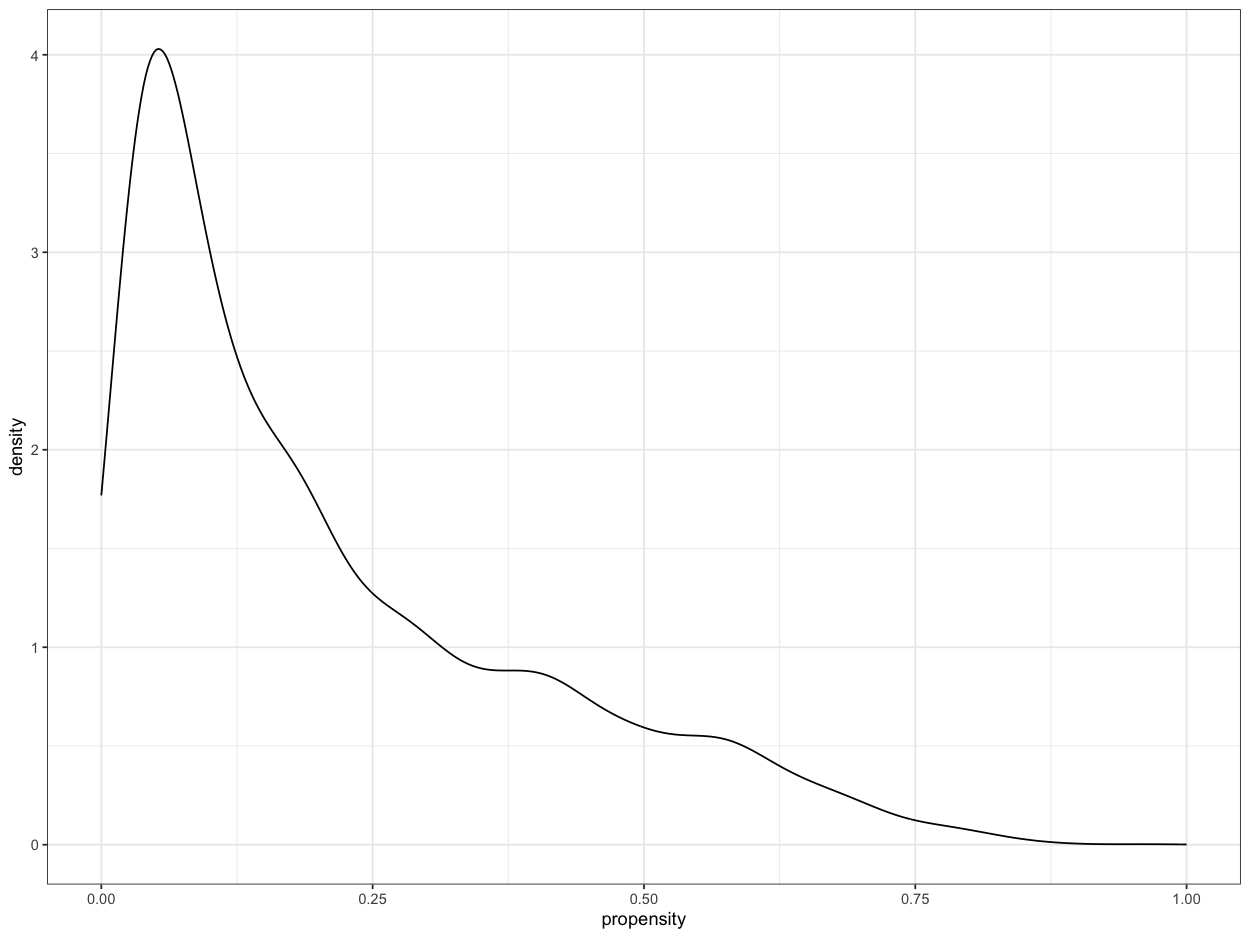
\includegraphics{out/propden.png}

}

\caption{\label{fig-propden2}Denstiy of Estimated Propensity Score of
One Child}

\end{figure}%

We assume unconfoundedness, that the mental health of the only children
is independent of being the only child conditioning on the whole set of
the covariates. We start by comparing the hypothesis test of zero ATE by
OLS estimation of the effect of being the only child with the hypothesis
test of zero CATE for all covariate values. Under the unconfoundedness
assumption, the ATEs on confidence, anxiety and desperation can be
estimated by regressing the mental health measures on the treatment and
covariates. The OLS estimates of the ATEs are \(-0.088\), \(0.005\) and
\(-0.067\) respectively, with the ATE on confidence and desperation
statistically significant at \(5\%\) level. The ATE estimates are
similar to those in the basic specification of \citet{wu2014only} with a
different set of covariates. Our proposed test statistics for the zero
CATE test are \(30.18\), \(34.02\), \(61.18\) with \(14\) degrees of
freedom for confidence, anxiety and desperation respectively and the
p-values are all smaller than \(0.01\). We conclude that for all three
mental health measures, at least for some covariate values, the CATE is
different from zero. The test results for anxiety give us an example of
the difference between the zero ATE test and zero CATE test. If a
researcher focused on the zero ATE test only, he/she would probably be
misled by the insignificance of the ATE on anxiety and ignore the
heterogeneity in the treatment effects.

\begin{table}

\caption{\label{tbl-ocptest}Test Results for the CATE on Mental Health
of the Only Children}

\centering{

\small
\centering
\begin{tabular}{cccccccc}
\hline
                            &            & \multicolumn{3}{c}{Zero CATE Tests}                 & \multicolumn{3}{c}{Constant CATE Tests}             \\
Method                      &            & Confidence      & Anxiety         & Desperation     & Confidence      & Anxiety         & Desperation     \\ \hline
\multirow{3}{*}{Projection} & Chi-square & 30.18           & 34.02           & 61.18           & 29.54           & 33.83           & 60.97           \\
                            & df         & 14              & 14              & 14              & 13              & 13              & 13              \\
                            & p-value    & \textless{}0.01 & \textless{}0.01 & \textless{}0.01 & \textless{}0.01 & \textless{}0.01 & \textless{}0.01 \\ \hline
\multirow{3}{*}{Crump et al.}      & Chi-square & 25.37           & 21.09           & 41.04           & 16.47           & 20.99           & 32.17           \\
                            & df         & 14              & 14              & 14              & 13              & 13              & 13              \\
                            & p-value    & 0.03           & 0.10           & \textless{}0.01 & 0.29            & 0.10            & \textless{}0.01 \\ \hline
\end{tabular}

}

\end{table}%

We then test the null hypothesis of constant CATE. The test statistics
for the three measures are \(29.54\), \(33.83\), \(60.97\) respectively
with \(13\) degrees of freedom and the null hypotheses of constant
treatment effect for all three measures are rejected at \(1\%\) level.
This suggests heterogeneous treatment effect of OCP on all three mental
health measures. We also compare our test with parametric test in
\citet{crump2008nonparametric}, which yields p-values \(0.03\),
\(0.10\), \(< 0.01\) for the three mental health measures in the test of
zero CATE and p-values \(0.29\), \(0.10\) and \(< 0.01\) in the test of
constant CATE.

We now show how to explore the source of treatment effect heterogeneity
using the CATE projection coefficients. Given that the ATE on anxiety is
not significant but heterogeneity is suggested by the hypothesis test,
we are interested in the subpopulations with positive or negative
treatment effects on the anxiety levels. Using the CATE projection
results in Table~\ref{tbl-modcate2}, we find that the only children with
older mother, lower maternal education, higher paternal education and
lower personal income are more anxious in general. Similar heterogeneity
analysis can be applied to the confidence and desperation of the
children using Table~\ref{tbl-confidencecate} and
Table~\ref{tbl-desperationcate}. We note that it should not be concluded
that a covariate is uncorrelated with the CATEs of OCP if it is
statistically insignificant in the second step regression. The
regression results show the partial effect of the covariates on the
CATE. When some of the covariates are mutually correlated, it is
possible to find a different subset of the covariates such that it is
almost equally predictive in the CATE.

\begin{table}

\caption{\label{tbl-modcate2}CATE Regression Results for Anxiety}

\centering{

\centering
\begin{threeparttable}
\begin{tabular}{lccc}
\hline
                            & Estimate & SE    & t test p-value \\ \hline
Intercept                   & 0.1892     & 0.3111  & 0.5433         \\
Age                         & 0.0024     & 0.0129  & 0.8506         \\
Urban                       & 0.1178     & 0.0677  & 0.0820.        \\
Gender                      & -0.0538    & 0.0640  & 0.4003         \\
Family Income               & -0.1193    & 0.0692  & 0.0849.        \\
Father Age                  & 0.0183     & 0.0101  & 0.0713.        \\
Mother Age                  & -0.0226    & 0.0119  & 0.0565.        \\
Father Edu Year             & -0.0203    & 0.0085  & 0.0173$^*$     \\
Mother Edu Year             & 0.0171     & 0.0081  & 0.0337$^*$     \\
Parents Divorce             & 0.1019     & 0.2627  & 0.6980         \\
Parents Remarriage          & -0.0765    & 0.5401  & 0.8874         \\
Han                         & -0.0514    & 0.1301  & 0.6929         \\ 
Marriage                    & 0.0490     & 0.0699  & 0.4838         \\ 
Personal Income             & 0.5844     & 0.1416  & 0.0000$^{***}$ \\ \hline
\end{tabular}
\begin{tablenotes}
\footnotesize
\item p-value 0 *** 0.001 ** 0.01 * 0.05 . 0.1
\item Family Income and Personal Income are scaled in $10^5$ CNY.
\end{tablenotes}
\end{threeparttable}

}

\end{table}%

\subsection{Testing the Effect of 401(k) Plans on Net Financial
Assets}\label{sec-retire}

The tax-deferred 401(k) plans\footnote{We use the \texttt{pension}
  dataset in \texttt{R} package \texttt{hdm}. More detailed description
  of this dataset can be found in \citet{chernozhukov2004effects} and
  \citet{belloni2017program}.} were introduced by the United States in
the early 1980s which aim to encourage employees to increase savings for
retirement through deducting contributions from taxable income and
tax-free accrual of interest. Employees' contributions may be matched by
the employers up to a certain percentage. 401(k) plans are provided by
employers, therefore, only the employees in the firms that offer 401(k)
plans are eligible. 401(k) plans are used for increasing retirement
savings, however, the effect of 401(k) plans on net financial assets is
less clear and this question has been studied by several papers in the
savings literature
\citep[e.g][]{poterba1995401, abadie2003semiparametric, chernozhukov2004effects}.

The key problem in determining the the effect of 401(k) plans on assets
is selection into participation. In order to deal with the selection
problem, we consider two identification strategies. First, we use 401(k)
eligibility as an instrument for 401(k) participating and assume
exogenous instrument conditioning on the basic covariates, which are
age, gender, income, family size, education years, marriage indicator,
two-earner indicator, defined benefit pension status indicator, IRA plan
participation indicator and home owner indicator. Second, we assume
unconfoundedness by including all basic covariates in the dataset, as
well as quadratic terms of age, income, family size, discretized income
category and full interactions. This leads to a total of \(211\)
covariates. With all basic and created covariates, we assume that
\(\mu_0(w, x)\) and \(e_0(x)\) are approximately sparse models where
\(\mu_0(w, x)\) is the potential outcomes of net financial assets and
\(e_0(x)\) is the propensity of 410(k) participation. For the first
strategy, we test the null hypothesis of constant CLATE using the method
in Section~\ref{sec-clatetest} and for the second strategy, we test the
null hypothesis of constant CATE in a high-dimensional setting using the
method in Section~\ref{sec-extend}.

Table~\ref{tbl-sum401k} presents descriptive statistics of the outcome,
treatment and basic covariates for the entire sample as well as
subgroups by participation status. The dataset contains 9915 units with
382 eligible for 401(k) plan and 2594 participated. The propensity of
eligibility \(q(x)\) is specified as a logit model with basic covariates
and the outcome regression models \(\mu^y_0(z, x)\) and
\(\mu^w_0(z, x)\) are estimated by OLS with \(z = 1, 0\) denoting the
eligibility status. Because non-eligible units are not allowed to
participate 401(k), so we let \(\hat\mu^w(0, x) = 0\) for all \(x\). We
also replace \(\hat\mu^w(1, x)\) greater than 1 with 1 to restrict the
probability of participation within \([0, 1]\). The test statistic
\(W_3\) in Equation~\ref{eq-wald3} is calculated to be \(51.57\) with
\(10\) degrees of freedom\footnote{Four observations are removed due to
  \(\hat{q}(x)\) close to \(1\).}. For the constant CLATE test, we get a
clear rejection at \(1\%\) level.

We then test the null hypothesis of constant CATE with high-dimensional
covariates under unconfoundedness assumption. We randomly split the
sample into \(K = 5\) subsets. The nuisance parameters \(\mu_0(w, x)\)
and \(e_0(x)\) are estimated by linear and logistic regressions with the
lasso respectively, with penalty level chosen according to
\citet{belloni2014high}. In the second step projection, \(b(X_i)\) is
chosen to be the baseline covariates. Using DML estimates of \(\beta_0\)
and the corresponding covariance matrix, the Wald statistic is
calculated to be \(83.35\) with \(10\) degrees of freedom, so the null
hypothesis of constant CATE is rejected at \(1\%\) level. Both our
statistical evidence of heterogeneous CLATE and CATE supports the
findings by \citet{chernozhukov2004effects}, who investigated the
heterogeneous treatment effect of 401(k) participation on net financial
assets using an instrumental quantile regression.

\section{Conclusion}\label{sec-conclude}

In this paper, we develop hypothesis tests for the existence of non-zero
and heterogeneous CATE/CLATE under the unconfoundedness and IV
identification by translating the hypotheses into the joint significance
of the BLP coefficients of the CATE/CLATE on the covariates. We propose
estimators of the BLP coefficients and derive the corresponding
asymptotic variance-covariance matrix. In contrast to existing methods,
our proposed parametric tests are straightforward to implement as the
test statistic can be constructed by the standard regression output in
statistical softwares. Semiparametric tests are developed to allow for
highly nonlinear models or high-dimensional covariates using
Double/Debiased Machine Learning estimators. Our proposed tests are
flexible as the CATE/CLATE can be tested on a function of covariates
such as a subset, polynomials or interactions without the need to change
the specifications of the outcome or propensity score. The finite sample
performance of the tests in terms of statistical power and size is
studied using Monte Carlo simulations. Finally, by applying the tests to
the survey data regarding One-child Policy and 401(k) retirement savings
plan, we find evidence of the presence of heterogeneous treatment
effects and illustrate the use of the estimated BLP coefficients for
subpopulation analysis.

\newpage

\section*{References}\label{references}
\addcontentsline{toc}{section}{References}

\renewcommand{\bibsection}{}
\bibliography{references.bib}

\newpage

\setcounter{section}{0}
\renewcommand{\thesection}{\Alph{section}}

\setcounter{table}{0}
\renewcommand{\thetable}{A\arabic{table}}

\setcounter{figure}{0}
\renewcommand{\thefigure}{A\arabic{figure}}

\section{Appendix}\label{appendix}

\subsection{Extra Results and Proofs}\label{sec-appenda}

\begin{proof}[Proof of Proposition~\ref{prp-consistency}]
Note that \(\hat\gamma \xrightarrow{p} \gamma_0\). We have \[
\hat\beta = (\frac1n\sum_{i = 1}^{n}(b(X_i)'b(X_i)))^{-1}(\frac1n\sum_{i = 1}^{n}(b(X_i)'Y^*_i(\hat\gamma))) \xrightarrow{p} G_\beta^{-1}\mathbb{E}[b(X_i)'Y^*_i(\gamma_0)] = \beta_0
\] as \(Y_i^*(\gamma)\) is continuous at \(\gamma_0\).
\end{proof}

\begin{proof}[Proof of Proposition~\ref{prp-main}]
The proof consists of two parts. First, we derive the asymptotic
variance of OLS estimator \(\hat\beta\) with plugged in nuisance
estimators \(\hat\gamma\). Second, we show how AIPW transformation
eliminates the influence of \(\hat\gamma\) on the asymptotic variance of
\(\hat\beta\). Note that \(\hat\gamma\) is an asymptotically linear
estimator with influence function \(\psi(d) = -M^{-1}m(d, \gamma_0)\)
where \(M = \mathbb{E}[\partial_\gamma m(D_i, \gamma_0)]\) and
\(\sqrt{n}(\hat\gamma - \gamma_0) = \sum_{i = 1}^{n}\psi(D_i)/\sqrt{n} + o_\text{p}(1)\).
Expanding \(\frac1n\sum_{i = 1}^{n}g(D_i, \beta, \hat\gamma) = 0\) and
solving with mean value theorem, we have
\begin{equation}\phantomsection\label{eq-pluginvar}{
\begin{aligned}
& \sqrt{n}(\hat\beta - \beta_0) \\
= & \left( \frac1n\sum_{i = 1}^{n} b(X_i)'b(X_i) \right)^{-1}\left(\frac{1}{\sqrt{n}}\sum_{i = 1}^{n} (b(X_i)'\epsilon_i + b(X_i)'\partial_\gamma Y_i^*(\bar\gamma)(\hat\gamma - \gamma_0)) \right) \\
= & \left( \frac1n\sum_{i = 1}^{n} b(X_i)'b(X_i) \right)^{-1}\left[ \frac{1}{\sqrt{n}}\sum_{i = 1}^{n}b(X_i)'\epsilon_i + \left( \frac1n\sum_{j = 1}^{n}b(X_j)'\partial_\gamma Y_j^*(\bar\gamma) \right) \sqrt{n}(\hat\gamma - \gamma_0) \right] \\
= & \left( \frac1n\sum_{i = 1}^{n} b(X_i)'b(X_i) \right)^{-1}\left[ \frac{1}{\sqrt{n}}\sum_{i = 1}^{n}b(X_i)'\epsilon_i + \frac{1}{\sqrt{n}} \sum_{i = 1}^{n} \left( \frac1n\sum_{j = 1}^{n} b(X_j)' \partial_\gamma Y_j^*(\bar\gamma)  \right) \psi(D_i) \right] + o_\text{p}(1) \\
= & \left( \frac1n\sum_{i = 1}^{n} b(X_i)'b(X_i) \right)^{-1}\left[ \frac{1}{\sqrt{n}} \sum_{i = 1}^{n} \left(b(X_i)'\epsilon_i +\left( \frac1n\sum_{j = 1}^{n} b(X_j)' \partial_\gamma Y_j^*(\bar\gamma) \right) \psi(D_i)\right)\right] + o_p(1)
\end{aligned}
}\end{equation} where \(\bar\gamma\) is the mean value. So
\(\sqrt{n}(\hat\beta - \beta_0) \xrightarrow{d} N(0, V)\) where
\(V = G_\beta^{-1}\mathbb{E}[(b(X_i)'\epsilon_i + G_\gamma \psi(D_i))(b(X_i)'\epsilon_i + G_\gamma\psi(D_i))']G_\beta^{-1}{'}\).

For \(g(d, \beta, \hat\gamma) = b(x)'(y^*(\hat\gamma) - b(x)\beta)\), we
have \[\begin{aligned}
G_\gamma &= \mathbb{E}[b(X_i)'(\partial_\gamma Y_i^*(\gamma_0))] \\
&= \mathbb{E}\left[b(X_i)'\mathbb{E}\left[\left(\left. \frac{W_i(\mu_0(1, X_i) - Y_i)}{e_0(X_i)^2} - \frac{(1 - W_i)(Y_i - \mu_0(0, X_i))}{(1 - e_0(X_i))^2}, \frac{e_0(X_i) - W_i}{1 - e_0(X_i)}, \frac{e_0(X_i) - W_i}{e_0(X_i)}\right) \right\vert X_i\right]\right] \\ 
&= 0.
\end{aligned}\] The last line holds by the definition of \(e_0(x)\),
\(\mu_0(w, x)\) and that
\(\mathbb{E}[W_i(Y_i - \mu_0(1, X_i))\vert X_i] = \mathbb{E}[(1 - W_i)(Y_i - \mu_0(0, X_i))\vert X_i] = 0\).
\end{proof}

\begin{proof}[Proof of Theorem~\ref{thm-cate} and
Theorem~\ref{thm-clate}]
Let \(p\)-dimensional vector \(\kappa\) represent BLP coefficients
\(\beta\) in the CATE tests/zero CLATE test, or \(r(\xi)\) in the
constant CLATE test. Proposition~\ref{prp-main} shows that
\(\sqrt{n}(\kappa - \kappa_0) \xrightarrow{d} Z \sim N(0, V_\kappa)\)
for some normal random vector \(Z\). Let
\(\hat{V}_\kappa \xrightarrow{p} V_\kappa\). Then it follows that \[
W = \sqrt{n}(\hat\kappa - \kappa_0)'\hat{V}_\kappa^{-1}\sqrt{n}(\hat\kappa - \kappa_0) \xrightarrow{d} Z'V_\kappa^{-1}Z \sim \chi^2_{p}.
\] Under the null hypothesis, \(\kappa_0 = 0\), therefore, \[
W = n\hat\kappa'\hat{V}_\kappa^{-1}\hat\kappa = \hat\kappa'(\hat{V}_\kappa / n)^{-1}\hat\kappa \xrightarrow{d} \chi^2_{p}.
\]
\end{proof}

\textbf{Double Robustness and Semiparametric Efficiency of the Estimator
of Projection Coefficients}

In the literature of causal inference, AIPW is largely known and used
for estimating the ATE using \(1/n\sum_i Y_i^*(\gamma)\). The AIPW
estimator of the ATE has attractive properties over the the OLS
estimator and the original IPW estimator
\citep[e.g.][]{scharfstein1999adjusting, lunceford2004stratification}.
Firstly, it is a doubly robust estimator which is consistent when either
\(e_0(X)\) or \(\mu_0(W, X)\) is correctly specified. Secondly, the
theory in \citet{robins1994estimation} guarantees that the AIPW
estimator of the ATE achieves the semiparametric efficiency. This result
is also shown in \citet{lunceford2004stratification} via simulations. In
this section, we show that our proposed \(\hat\beta\) with AIPW
transformation, which is an estimator of the projection coefficients of
\(Y_i^*(\gamma)\) on the covariates, inherits these properties. To
formally define double robustness, we introduce additional notations as
follows. By the parametric setting of \(e(X)\) and \(\mu(W, X)\), let
\(e(X, \gamma_{e_0}) = e_0(X)\),
\(\mu(X, \gamma^1_{\mu_0}) = \mu_0(1, X)\) and
\(\mu(X, \gamma^0_{\mu_0}) = \mu_0(0, X)\). If \(\mu(W, X)\) is
correctly specified, we have
\(\hat\gamma^w_\mu \xrightarrow{p} \gamma^w_{\mu_0}\) and \[
\mu(X, \hat\gamma^w_\mu) \xrightarrow{p} \mu_0(w, X) = \mathbb{E}[Y(w)|X]
\] for \(w = 0, 1\), whereas if \(\mu(W, X)\) is misspecified, then
\(\hat\gamma^w_\mu \xrightarrow{p} \gamma^w_{\tilde\mu}\) and \[
\mu(X, \hat\gamma^w_\mu) \xrightarrow{p} \tilde\mu(w, X) \neq \mathbb{E}[Y(w)|X].
\] Similarly, if \(e(X)\) is correctly specified, we have
\(\hat\gamma_e \xrightarrow{p} \gamma_{e_0}\) and \[
e(X, \hat\gamma_e) \xrightarrow{p} e_0(X) = P(W = 1|X)
\] whereas if misspecified,
\(\hat\gamma_e \xrightarrow{p} \gamma_{\tilde{e}}\) and \[
e(X, \hat\gamma_e) \xrightarrow{p} \tilde{e}(X) \neq P(W = 1|X).
\]

\begin{proposition}[Double
Robustness]\protect\hypertarget{prp-doublerobust}{}\label{prp-doublerobust}

Suppose the assumptions stated in Proposition~\ref{prp-main} is
satisfied. \(\hat\beta \xrightarrow{p} \beta_0\) when
\(\hat\gamma^w_\mu \xrightarrow{p} \gamma^w_{\mu_0}\) or
\(\hat\gamma_e \xrightarrow{p} \gamma_{e_0}\).

\end{proposition}

\begin{proof}
Decompose \(\hat\beta\) by Equation~\ref{eq-tot} and consider the
component \[
(\frac1n\sum_{i = 1}^{n}(b(X_i)'b(X_i)))^{-1}\frac1n\sum_{i = 1}^{n}\left(b(X_i)'\left(D_i\frac{Y_i - \mu(X_i, \hat\gamma^1_\mu))}{e(X_i, \hat\gamma_e)} + \mu(X_i, \hat\gamma^1_\mu)\right)\right).
\] Suppose only \(\mu(W, X)\) is correctly specified and by
\(W_iY_i = W_iY_i(1)\), then this component can be written as
\begin{equation}\phantomsection\label{eq-ytreat}{
(\frac1n\sum_{i = 1}^{n}(b(X_i)'b(X_i)))^{-1}\frac1n\sum_{i = 1}^{n}\left(b(X_i)'\left(Y_i(1) + \frac{W_i - \tilde{e}(X_i)}{\tilde{e}(X_i)}(Y_i(1) - \mathbb{E}[Y_i(1)|X_i])\right)\right) + o_p(1)
}\end{equation} which converges to \[
\begin{aligned}
G_\beta^{-1}&\mathbb{E}[b(X_i)'Y_i(1)] + G_\beta^{-1}\mathbb{E}\left[b(X_i)'\frac{W_i - \tilde{e}(X_i)}{\tilde{e}(X_i)}(Y_i(1) - \mathbb{E}[Y_i(1)|X_i]\right] \\
= G_\beta^{-1}&\mathbb{E}[b(X_i)'Y_i(1)] + G_\beta^{-1}\mathbb{E}\left[b(X_i)'\frac{W_i - \tilde{e}(X_i)}{\tilde{e}(X_i)}\mathbb{E}[Y_i(1) - \mathbb{E}[Y_i(1) \vert X_i] \vert W_i, X_i]\right] \\
= G_\beta^{-1}&\mathbb{E}[b(X_i)'Y_i(1)]
\end{aligned}
\] where the second equation follows by the law of iterated expectations
conditioning on \(W_i\) and \(X_i\). Similarly, the other component in
\(\hat\beta\) converges to \(-G_\beta^{-1}\mathbb{E}[b(X_i)Y_i(0)]\).
Thus,
\(\hat\beta \xrightarrow{p} \beta_0 = G_\beta^{-1}\mathbb{E}[b(X_i)'(Y_i(1) - Y_i(0))]\).

Suppose only \(e(X)\) is correctly specified, then
Equation~\ref{eq-ytreat} converges to \[
\begin{aligned}
&G_\beta^{-1}\mathbb{E}[b(X_i)'Y_i(1)] + G_\beta^{-1}\mathbb{E}\left[b(X_i)'\frac{W_i - p(W_i = 1|X_i)}{p(W_i = 1|X_i)}(Y_i - \tilde{\mu}(1, X_i))\right] \\
= &G_\beta^{-1}\mathbb{E}[b(X_i)'Y_i(1)] + G_\beta^{-1}\mathbb{E}[b(X_i)'\frac{\mathbb{E}[W_i|Y_i(1), X_i] - P(W_i = 1|X_i)}{P(W_I = 1|X_i)}(Y_i(1) - \tilde{\mu}(1, X_i))] \\
= &G_\beta^{-1}\mathbb{E}[b(X_i)'Y_i(1)]
\end{aligned}
\] where the second equation follows by the law of iterated expectations
conditioning on \(Y_i(1)\) and \(X_i\). Similarly, we can derive the
probability limit of the other component in \(\hat\beta\) and then
\(\hat\beta \xrightarrow{p} \beta_0\).
\end{proof}

Next we employ the theory of semiparametric efficient influence function
to show that \(\hat\beta\) is a locally efficient semiparametric
estimator. This property of \(\hat\beta\) guarantees that our proposed
hypothesis tests for the CATE/CLATE have more statistical power than
other semiparametric estimators of \(\beta_0\).

\begin{proposition}[Semiparametric
Efficiency]\protect\hypertarget{prp-efficiency}{}\label{prp-efficiency}

\(\hat\beta\) is locally efficient in the class of regular and
asymptotically linear estimators of \(\beta_0\).

\end{proposition}

\begin{proof}
We refer to \(D_i^F = (Y_i(1), Y_i(0), X_i)\) as the full data. Let
\(\Phi\) denote the space of observed data influence functions of
regular and asymptotically linear estimators of \(\beta_0\), and
\(\Phi^F\) denote the space of full data influence functions. By the
theory of missing data influence function, there is a many-to-one linear
function \(\mathcal{K}: \ \Phi \rightarrow \Phi^F\), where for any
\(\varphi \in \Phi\),
\(\mathcal{K}(\varphi(D_i)) = \mathbb{E}[\varphi(D_i)|D_i^F]\).
Therefore \(\mathcal{K}^{-1}(\varphi^F(D_i^F))\) denotes all the
functions \(\varphi(D_i)\) such that \[
\mathbb{E}[\varphi(D_i)|D_i^F] = \varphi^F(D_i^F)
\] Thus, for any function \(\varphi(D_i)\) that satisfies this
condition, the class of observed data influence function
\(\mathcal{K}^{-1}[\varphi^F(D_i^F)]\) is equal to
\(\varphi(D_i) + L(D_i)\) where \(L \in \mathcal{L}\) is a linear
subspace in \(\Phi\) such that \(\mathbb{E}[L(D_i)|D_i^F] = 0\).

For \(\beta_0\),
\(\varphi^F(D_i^F) = G_\beta^{-1}b(X_i)'(Y_i(1) - Y_i(0) - b(X_i)\beta_0)\).
By our previous discussion, one of such functions \(\varphi(D_i)\),
motivated by IPW, is \begin{equation}\phantomsection\label{eq-ipwif}{
\varphi(D_i) = G_\beta^{-1}b(X_i)'\left(\frac{W_iY_i}{e_0(X_i)} - \frac{(1 - W_i)Y_i}{1 - e_0(X_i)} - b(X_i)\beta_0\right).
}\end{equation} Because \(W_i\) is a dummy variable, then we have
\begin{equation}\phantomsection\label{eq-lf}{
L(D_i) = L(Y_i, W_i, X_i) = W_iL_1(Y_i, X_i) + (1 - W_i)L_0(Y_i, X_i)
(\#eq:lf)
}\end{equation} for some functions \(L_1(\cdot)\) and \(L_0(\cdot)\) and
thus, \[
\mathbb{E}[L(D_i)|D_i^F] = e_0(X)L_1(Y_i(1), X_i) + (1 - e_0(X_i))L_0(Y_i(0), X_i) = 0.
\] The second equation suggests \[
L_0(Y_i(0), X_i) = -\frac{e_0(X_i)}{1 - e_0(X_i)}L_1(Y_i(0), X_i).
\] For this equation to hold, \(L_1(\cdot)\) and \(L_0(\cdot)\) must be
functions of \(X_i\) only. Combining this equation with
Equation~\ref{eq-lf}, \(\mathcal{L}\) consists of functions \[
\left(\frac{W - e_0(X_i)}{1 - e_0(X_i)}\right)L_1(X_i) \ \text{for some function} \ L_1(X_i)
\] or equivalently, \(\mathcal{L}\) consists of functions \[
(W - e_0(X_i))L_2(X_i) \ \text{for some function} \ L_2(X_i).
\]

Therefore, The efficient influence function can be obtained by \[
\varphi(D_i) - (W_i - e_0(X_i))L^p_2(X_i)
\] where \(L^p_2(X_i)\) satisfies \[
\mathbb{E}[(\varphi(D_i) - (W_i - e_0(X_i))L^p_2(X_i)))(W_i - e_0(X_i))L_2(X_i)] = 0
\] for all \(L_2(X_i) \in \mathcal{L}\).

Let \(\Pi[\varphi(D_i)|\mathcal{L}] = (W_i - e_0(X_i))L^p_2(X_i)\)
denote the projection of \(\varphi(D_i)\) on \(\mathcal{L}\). We have
\begin{equation}\phantomsection\label{eq-projphi}{
\Pi[\varphi(D_i)|\mathcal{L}] = \Pi[W_i\varphi_1(Y_i, X_i)|\mathcal{L}] + \Pi[(1 - W_i)\varphi_0(Y_i, X_i)|\mathcal{L}].
}\end{equation} Consider the first term on the RHS, we have the
condition \[
\mathbb{E}[(W_i\varphi_1(Y_i, X_i) - (W_i - e_0(X_i))L^p_{21}(X_i)))(W_i - e_0(X_i))L_2(X_i)] = 0 
\] or equivalently \[
\mathbb{E}[W_i(W_i - e_0(X_i))L_2(X_i)\varphi_1(Y_i, X_i)] - \mathbb{E}[(W_i - e_0(X_i))^2L^p_{21}(X_i)L_2(X_i)] = 0.
\] By the law of iterated expectations twice, the first term on the LHS
is equal to \[
\begin{aligned}
&\mathbb{E}[\mathbb{E}[W_i(W_i - e_0(X_i))L_2(X_i)\varphi_1(Y_i, X_i)|W_i, X_i]] \\
= &\mathbb{E}[W_i(W_i - e_0(X_i))L_2(X_i)\mathbb{E}[\varphi_1(Y_i, X_i)|W_i = 1, X_i]] \\
= &\mathbb{E}[\mathbb{E}[W_i(W_i - e_0(X_i))L_2(X_i)\mathbb{E}[\varphi_1(Y_i, X_i)|W_i = 1, X_i]|X_i]] \\
= &\mathbb{E}[e_0(X_i)(1 - e_0(X_i))L_2(X_i)\mathbb{E}[\varphi(Y_i, X_i)|W_i = 1, X_i]]
\end{aligned}
\] and the second term on the RHS is equal to \[
\begin{aligned}
\mathbb{E}&[\mathbb{E}[(W_i - e_0(X_i))^2|X_i]L^p_{21}(X_i)L_2(X_i)] \\
= \mathbb{E}&[Var(W_i|X_i)L^p_{21}(X_i)L_2(X_i)] \\
= \mathbb{E}&[e_0(X_i)(1 - e_0(X_i))L^p_{21}(X_i)L_2(X_i)].
\end{aligned}
\] Therefore, \[
\mathbb{E}[e_0(X_i)(1 - e_0(X_i))(\mathbb{E}[\varphi_1(Y_i, X_i)|W_i = 1, X_i] - L^p_{21}(X_i))L_2(X_i)] = 0
\] for all \(L_2(X_i) \in \mathcal{L}\). So this equation holds if and
only if \[
L^p_{21}(X_i) = \mathbb{E}[\varphi_1(X_i)|W_i = 1, X_i].
\] Similarly, we can prove that
\(L^p_{20}(X_i) = -\mathbb{E}[\varphi_0(X_i)|W_i = 0, X_i]\) for the
second term in Equation~\ref{eq-projphi}.

By the arguments above, the efficient influence function is \[
\varphi(D_i) - \Pi(\varphi(D_i)|\mathcal{L}) = G_\beta^{-1}b(X_i)'\left(Y_i^*(\gamma_0) - b(X_i)\beta_0\right).
\] As \(\mu_0(w, x)\) and \(e_0(x)\) are usually unknown in practice,
substituting in consistent estimators of \(\hat\mu_0(w, x)\) and
\(\hat{e}_0(x)\), we have the corresponding locally efficient estimator
\(\hat\beta\) described in Proposition~\ref{prp-consistency}
\end{proof}

It is worth noting that the estimated projection coefficient with IPW
transformation has the same asymptotic variance as the AIPW
transformation when the propensity score is unknown. However, AIPW
transformation is asymptotically more efficient when the propensity
score is known, for example, in a randomized experiment where propensity
score is a known constant by design. It is not difficult to prove this
claim using the proof for Proposition~\ref{prp-efficiency}. If
\(e_0(X_i)\) is known, the influence function for \(\hat\beta\) with IPW
transformation is given by Equation~\ref{eq-ipwif}, which is not
efficient. If \(e_0(X_i)\) is unknown, \((W_i - e_0(X_i))L^p_2(X_i)\)
serves as a correction term capturing the effect of estimating
\(e_0(X_i)\) on the influence function of IPW. This is an extension of
the discussion in \citet{hirano2003efficient} to the projection
coefficients of conditional treatment effects. Moreover, AIPW
transformation provides smaller variance than IPW in finite samples.
Hence, AIPW transformation is preferable to IPW.

\begin{proof}[Proof of Proposition~\ref{prp-dml}]
Observe that the moment function in Equation~\ref{eq-moment0} is a
linear in \(\beta\), where \[
g(d, \beta, \gamma) = g^b(d, \gamma) + g^a(d, \gamma)\beta = b(x)'y^*(\gamma) - b(x)'b(x)\beta
\] and Proposition~\ref{prp-dml} follows from Theorems 3.1 and 3.2 and
Corollary 3.1 in \citet{chernozhukov2018double} as long as we can verify
Assumptions 3.1 and 3.2 in \citet{chernozhukov2018double}. We proceed in
3 steps as follows. Step 1 verifies Neyman-orthogonality of the moment
function. Step 2 verifies the regularity conditions of the moment
function in required in Assumption 3.1. Step 3 shows the construction of
the realization set \(\mathcal{T}_n\) and verifies Assumption 3.2.

Step 1.

\[
\begin{aligned}
&\partial_r \mathbb{E}[g(D_i, \beta_0, \gamma_0 + r(\gamma - \gamma_0))]\vert_{r = 0} \\
= & \mathbb{E}[b(X_i)'(\mu(1, X_i) - \mu_0(1, X_i) - \mu(0, X_i) + \mu_0(0, X_i))] \\
- &\mathbb{E}\left[b(X_i)'\left(\frac{W_i(\mu(1, X_i) - \mu_0(1, X_i))}{e_0(X_i)} - \frac{(1 - W_i)(\mu(0, X_i) - \mu_0(0, X_i))}{1 - e_0(X_i)}\right)\right] \\
- &\mathbb{E}\left[b(X_i)'\left(\frac{W_i(Y - \mu_0(1, X_i))(e(X_i) - e_0(X_i))}{e^2(X_i)} - \frac{(1 - W_i)(Y_i - \mu_0(0, X_i))(e(X_i) - e_0(X_i))}{(1 - e_0(X_i))^2}\right)\right] \\
= & \mathbb{E}[b(X_i)'(\mu(1, X_i) - \mu_0(1, X_i) - \mu(0, X_i) + \mu_0(0, X_i))] \\
- &\mathbb{E}\left[b(X_i)'\left(\frac{\mathbb{E}[W_i|X_i](\mu(1, X_i) - \mu_0(1, X_i))}{e_0(X_i)} - \frac{\mathbb{E}[(1 - W_i)|X_i](\mu(0, X_i) - \mu_0(0, X_i))}{1 - e_0(X_i)}\right)\right] \\
- &\mathbb{E}\left[b(X_i)'\left(\frac{\mathbb{E}[W_i(Y - \mu_0(1, X_i))|X_i](e(X_i) - e_0(X_i))}{e^2(X_i)}\right)\right] \\
- &\mathbb{E}\left[b(X_i)'\left(\frac{\mathbb{E}[(1 - W_i)(Y_i - \mu_0(0, X_i))|X_i](e(X_i) - e_0(X_i))}{(1 - e_0(X_i))^2}\right)\right] \\
= &0.
\end{aligned}
\] The second equation holds by the law of iterated expectation, and the
third equation holds by that
\(\mathbb{E}[W_i(Y_i - \mu_0(1, X_i))|X_i] = \mathbb{E}[(1 - W_i)(Y_i - \mu_0(0, X_i))|X_i] = 0\).
This gives Assumption 3.1(d) with exact Neyman-orthogonality
(\(\lambda_n\) = 0)

Step 2.

Assumption 3.1(e) in \citet{chernozhukov2018double} is given by
Assumption~\ref{exr-dml} (iii). And given that Assumption 3.1(a)-(c)
holds trivially, all conditions in Assumption 3.1 are satisfied.

Step 3.

The variance of the moment function \[
\mathbb{E}[g(D, \beta_0, \gamma_0)g(D, \beta_0, \gamma_0)'] = \mathbb{E}[b(X)'b(X)(Y^*(\gamma_0) - b(X)\beta)^2]
\] is positive definite by Assumption~\ref{exr-dml} (iv), so there
exists a positive value \(\underline{c}\) such that all eigenvalues of
\(\mathbb{E}[g(D, \beta_0, \gamma_0)g(D, \beta_0, \gamma_0)']\) are
bounded from below by \(\underline{c}\). This gives Assumption 3.2(d) as
long as \(c_0 \leqslant \underline{c}\).

Next, we verify the rest of Assumption 3.2 with \(\gamma = (\mu, e)\) in
the set \(\mathcal{T}_n\) such that \[
\begin{aligned}
\Vert \gamma - \gamma_0 \Vert_{F, q} &\leqslant C, \\
\Vert \gamma - \gamma_0 \Vert_{F, 2} &\leqslant \delta_n, \\
\Vert m - 1/2 \Vert_{F, \infty} &\leqslant 1/2 - \xi, \\
\Vert \mu - \mu_0 \Vert_{F, 2} \times \Vert e - e_0 \Vert_{F, 2} &\leqslant \delta_n n^{-1/2}.
\end{aligned}
\] And we replace the sequence \((\delta_n)_{n \geqslant 1}\) in
Assumption 3.2 by \((\delta'_n)_{n \geqslant 1}\) with
\(\delta'_n = C_\xi(\delta_n \vee N^{(-(1 - 4/q))\wedge(1/2)})\) where
\(C_\xi\) is some constant that depends only on \(\xi\) and \(C\). Note
that \(\delta'_n \geqslant N^{(-(1 - 4/q))\wedge(1/2)}\), which is
required in Theorems 3.1 and 3.2 in \citet{chernozhukov2018double}.

We have \[
\begin{aligned}
\Vert \mu_0(W, X) \Vert_{F, q} &= (\mathbb{E}[\vert \mu_0(W, X) \vert^q])^{1/q} \\
&\geqslant (\mathbb{E}[\vert \mu_0(1, X) \vert^q e_0(X) + \vert \mu_0(0, X) \vert^q (1 - e_0(X))])^{1/q} \\
&\geqslant \xi^{1/q}(\mathbb{E}[\vert \mu_0(1, X) \vert^q] + \mathbb{E}[\vert \mu_0(0, X) \vert^q])^{1/q} \\
&\geqslant \xi^{1/q}(\mathbb{E}[\vert \mu_0(1, X) \vert^q] \vee \mathbb{E}[\vert \mu_0(W, X) \vert^q])^{1/q} \\
&\geqslant \xi^{1/q}(\Vert \mu_0(1, X) \Vert_{F, q} \vee \Vert \mu_0(0, X) \Vert_{F, q})
\end{aligned}
\] where the third line holds by
\(\xi \leqslant e_0(X) \leqslant 1 - \xi\) in
Assumption~\ref{exr-overlap}. Given that
\(\Vert \mu_0(W, X) \Vert_{F, q} \leqslant \Vert Y \Vert_{F, q} \leqslant C\)
in Assumption~\ref{exr-dml} (i), we have \[
\Vert \mu_0(1, X) \Vert_{F, q} \leqslant C/\xi^{1/q} \quad \text{and} \quad \Vert \mu_0(0, X) \Vert_{F, q} \leqslant C/\xi^{1/q}.
\] Following a similar procedure, it can be shown that for any
\(\gamma \in \mathcal{T}_n\) \[
\Vert \mu(1, X) - \mu_0(1, X) \Vert_{F, q} \leqslant C/\xi^{1/q} \quad \text{and} \quad \Vert \mu(0, X) - \mu_0(0, X) \Vert_{F, q} \leqslant C/\xi^{1/q}
\] Then we have \[
\begin{aligned}
&\Vert Y^*(\gamma) \Vert_{F, q} = \left\Vert \frac{W(Y - \mu(1, X))}{e(X)} - \frac{(1 - W)(Y - \mu(0, X))}{1 - e(X)} + \mu(1, X) - \mu(0, X) \right\Vert_{F, q} \\
&\leqslant \xi^{-1}(\Vert Y \Vert_{F, q} + \Vert Y \Vert_{F, q} + \Vert \mu(1, X) \Vert_{F, q} + \Vert \mu(0, X) \Vert_{F, q}) + \Vert \mu(1, X) \Vert_{F, q} + \Vert \mu(0, X) \Vert_{F, q} \\
&\leqslant (1 + \xi^{-1})(\Vert \mu(1, X) - \mu_0(1, X) \Vert_{F, q} + \Vert \mu(0, X) - \mu_0(0, X) \Vert_{F, q} \\
&\quad + \Vert \mu_0(1, X) \Vert_{F, q} + \Vert \mu_0(0, X) \Vert_{F, q}) + 2\xi^{-1}\Vert Y \Vert_{F, q} \\
&\leqslant 4C(1 + \xi^{-1}) / \xi^{1/q} + 2C\xi^{-1}
\end{aligned}
\] where the second line and the third line hold by the triangular
inequality. Moreover, \begin{equation}\phantomsection\label{eq-yerror}{
\Vert Y^*(\gamma) - Y^*(\gamma_0) \Vert_{F, q} \leqslant \mathcal{I}_1 + \mathcal{I}_2 + \mathcal{I}_3
}\end{equation} where \[
\begin{aligned}
&\mathcal{I}_1 = \Vert \mu(1, X) - \mu_0(1, X) \Vert_{F, q} + \Vert \mu(0, X) - \mu_0(0, X) \Vert_{F, q} \\
&\mathcal{I}_2 = \left\Vert \frac{W(Y - \mu(1, X))}{e(X)} - \frac{W(Y - \mu_0(1, X))}{e_0(X)} \right\Vert_{F, q} \\
&\mathcal{I}_3 = \left\Vert \frac{(1 - W)(Y - \mu(0, X))}{1 - e(X)} - \frac{(1 - W)(Y - \mu_0(0, X))}{1 - e_0(X)} \right\Vert_{F, q}.
\end{aligned}
\]

We have \(\mathcal{I}_1 \leqslant 2C/\xi^{1/q}\) and \[
\begin{aligned}
\mathcal{I}_2 &\leqslant \xi^{-2}\Vert We_0(X)(Y - \mu(1, X)) - We(X)(Y - \mu_0(1, X)) \Vert_{F, q} \\
&\leqslant \xi^{-2} \Vert e_0(X)(U + \mu_0(1, X) - \mu(1, X)) - e(X)U \Vert_{F, q} \\
&\leqslant \xi^{-2} (\Vert e_0(X)(\mu(1, X) - \mu_0(1, X)) \Vert_{F, q} + \Vert U(e(X) - e_0(X)) \Vert_{F, q}) \\
&\leqslant \xi^{-2} (\Vert \mu(1, X) - \mu_0(1, X) \Vert_{F, q} + C^{1/q}\Vert e(X) - e_0(X) \Vert_{F, q}) \\
&\leqslant \xi^{-2}C(\xi^{-1/q} + C^{1/q})
\end{aligned}
\] where the second inequality follows from that \(W \in  \{0, 1\}\) and
\(Y = \mu_0(1, X) + U\) when \(W = 1\), the fourth line follows from the
fact that \(e_0(X) \leqslant 1\) and Assumption~\ref{exr-dml} (iv).
Similarly, \(\mathcal{I}_3 \leqslant \xi^{-2}C(\xi^{-1/q} + C^{1/q})\)
and thus,
\(\Vert Y^*(\gamma) - Y^*(\gamma_0) \Vert_{F, q} \leqslant 2C(\xi^{-1/q} + \xi^{-2 - 1/q} + \xi^{-2}C^{1/q})\).

Notice that \[\begin{aligned}
(\mathbb{E}[ \Vert g(D, \beta_0, \gamma) \Vert^{q}])^{1/q} &= \mathbb{E}[\Vert b(X)'(Y^*(\gamma) - b(X)\beta_0) \Vert^q]^{1/q} \\
&\leqslant C\Vert Y^*(\gamma) - b(X)\beta_0 \Vert_{F, q} \\
&= C(\Vert Y^*(\gamma) - Y^*(\gamma_0) + Y^*(\gamma_0) - b(X)\beta_0 \Vert_{F, q}) \\
&\leqslant C(\Vert Y^*(\gamma) - Y^*(\gamma_0) \Vert_{F, q} + \Vert Y^*(\gamma_0) - b(X)\beta_0 \Vert_{F, q}) \\
&\leqslant 2C^2(\xi^{-1/q} + \xi^{-2 - 1/q} + \xi^{-2}C^{1/q}) + C^2
\end{aligned}\] where the fourth line follows from
Assumption~\ref{exr-dml} (iv). This gives the bound on \(m_n\) in
Assumption 3.2(b). The bound on \(m'_n\) is given by
Assumption~\ref{exr-dml} (i) because the maximal eigenvalue of
\(b(X)'b(X)\) equals \(\Vert b(X) \Vert\).

At last, we verify Assumption 3.2(c) in \citet{chernozhukov2018double}.
\[
\Vert \mathbb{E}[g^a(D, \gamma)] - \mathbb{E}[g^a(D, \gamma_0)] \Vert = \Vert b(X)'b(X) - b(X)'b(X) \Vert = 0 \leqslant \delta'_n
\] which gives the bound on \(r_n\).

Notice that \[
(\mathbb{E}[\Vert g(D, \beta_0, \gamma) - g(D, \beta_0, \gamma_0) \Vert^2])^{1/2} = (\mathbb{E}[\Vert b(X) \Vert^2 \vert Y^*(\gamma) - Y^*(\gamma_0) \vert^2])^{1/2} \leqslant C \Vert Y^*(\gamma) - Y^*(\gamma_0) \Vert_{F, 2}.
\] Thus, to show the bound on \(r'_n\), it suffices to show the bound on
\(\Vert Y^*(\gamma) - Y^*(\gamma_0) \Vert_{F, 2}\). Similar to the steps
used in deriving the bound on Equation~\ref{eq-yerror} and that \[
\Vert \mu(1, X) - \mu_0(1, X) \Vert_{F, 2} \leqslant \delta_n/\xi^{1/2} \quad \text{and} \quad \Vert \mu(0, X) - \mu_0(0, X) \Vert_{F, 2} \leqslant \delta_n/\xi^{1/2},
\] we have
\(\Vert Y^*(\gamma) - Y^*(\gamma_0) \Vert_{F, 2} \leqslant 2(\xi^{-1/2} + \xi^{-5/2} + \sqrt{C}\xi^{-2})\delta_n\),
which gives \[
r'_n \leqslant 2C(\xi^{-1/2} + \xi^{-5/2} + \sqrt{C}\xi^{-2})\delta_n \leqslant \delta'_n
\] as long as \(C_\xi\) in the definition of \(\delta'_n\) satisfies
\(C_\xi \geqslant 2C(\xi^{-1/2} + \xi^{-5/2} + \sqrt{C}\xi^{-2})\).

Finally, let \[
f(r) = \mathbb{E}[g(D, \beta_0, \gamma_0 + r(\gamma - \gamma_0))], \quad r \in (0, 1).
\] Then \[
\begin{aligned}
\partial^2_r f(r) &= \partial_r^2 \mathbb{E}[b(X)'(Y^*(\gamma_0 + r(\gamma - \gamma_0))) - b(X)\beta_0] \\
&= 2\mathbb{E}\left[b(X)'\frac{W(\mu(1, X) - \mu_0(1, X))(e(X) - e_0(X))}{(e_0(X) + r(e(X) - e_0(X)))^2}\right] \\
&\quad + 2\mathbb{E}\left[b(X)'\frac{W(e(X) - e_0(X))^2(Y - \mu_0(1, X) - r(\mu(1, X) - \mu_0(1, X)))}{(e_0(X) + r(e(X) - e_0(X)))^3}\right] \\
&\quad + 2\mathbb{E}\left[b(X)'\frac{(1 - W)(\mu(0, X) - \mu_0(0, X))(e(X) - e_0(X)}{(1 - e_0(X) - r(e(X) - e_0(X))^2}\right] \\
&\quad - 2\mathbb{E}\left[b(X)'\frac{(1 - W)(e(X) - e_0(X))^2(Y - \mu_0(X) - r(\mu(X) - \mu_0(X)))}{(1 - e_0(X) - r(e(X) - e_0(X))^3}\right].
\end{aligned}
\] By similar arguments used in previous steps and given that \[
W(Y - \mu_0(1 , X)) = WU, \quad (1 - W)(Y - \mu_0(0, X)) = (1 - W)U, \quad \mathbb{E}[U|W, X] = 0, \quad |e(X) - e_0(X)| \leqslant 2
\] for some constant \(C'_\xi\) that depends only on \(\xi\) and \(C\),
\[
|\partial^2_r f(r)| \leqslant C'_\xi \Vert \mu - \mu_0 \Vert_{F, 4} \times \Vert e - e_0 \Vert_{F, 4} \leqslant \delta'_nn^{-1/2}
\] as long as \(C_\xi \geqslant C'_\xi\). This gives bound on
\(\lambda'_n\).

Thus all conditions of Assumption 3.1 and 3.2 in
\citet{chernozhukov2018double} are verified and this completes the
proof.
\end{proof}

\newpage

\subsection{Tables and Figures}\label{sec-appendb}

\blandscape

\begin{figure}

\centering{

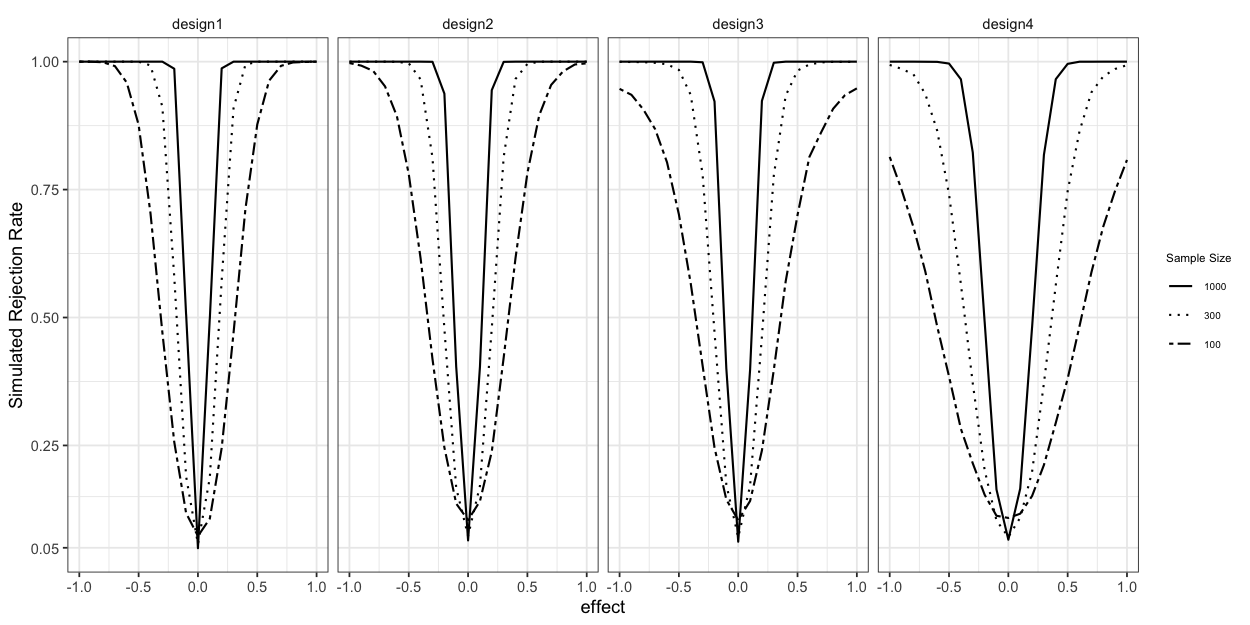
\includegraphics{out/p1.png}

}

\caption{\label{fig-power}Simulated Power of Test of Constant Treatment
Effect}

\end{figure}%

\elandscape

\newpage

\blandscape

\begin{figure}

\centering{

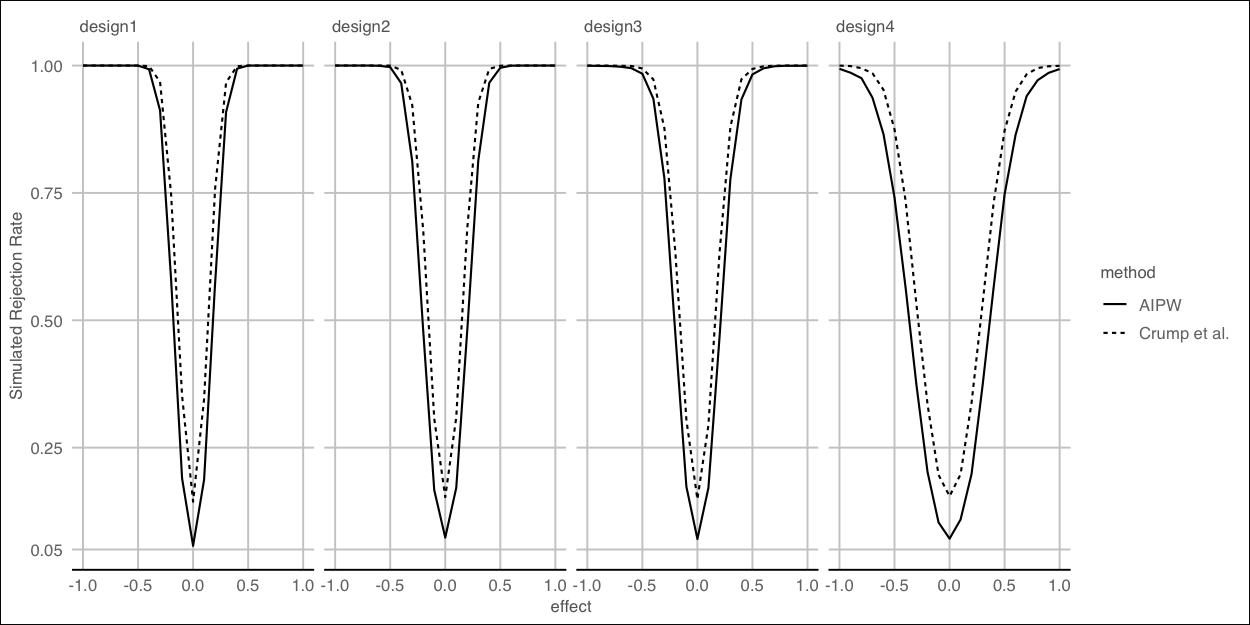
\includegraphics{out/compare.png}

}

\caption{\label{fig-compare}Comparison with Existing Parametric tests}

\end{figure}%

\elandscape

\newpage

\begin{table}

\caption{\label{tbl-sumonechild}Descriptive Statistics of CFPS Data}

\centering{

\centering
\begin{threeparttable}
\begin{tabular}{llll}
\hline
                            & Entire Sample & One-Child    & Non-One-Child \\ \hline
Onechild                    & 0.25          &              &                  \\
                            & (0.44)        &              &                  \\
Confidence                  & 4.00          & 3.94         & 4.03             \\
                            & (0.94)        & (0.93)       & (0.97)           \\
Anxiety                     & 4.62          & 4.62         & 4.62             \\
                            & (0.68)        & (0.68)       & (0.68)           \\
Desperation                 & 4.71          & 4.66         & 4.73             \\
                            & (0.62)        & (0.68)       & (0.60)           \\
Age                         & 26.15         & 25.71        & 26.31            \\
                            & (4.33)        & (3.95)       & (4.44)           \\
Urban                       & 0.61          & 0.82         & 0.54             \\
                            & (0.49)        & (0.38)       & (0.50)           \\
Gender                      & 0.55          & 0.61         & 0.53             \\
                            & (0.50)        & (0.49)       & (0.50)           \\
Family Income               & 46182.69      & 59046.11     & 41806.08         \\
                            & (50851.04)    & (59205.72)   & (46888.77)       \\
Father Age                  & 53.23         & 52.52        & 53.48            \\
                            & (6.47)        & (5.66)       & (6.71)           \\
Mother Age                  & 51.34         & 50.75        & 51.54            \\
                            & (6.01)        & (5.38)       & (6.21)           \\
Father Edu Year             & 7.57          & 8.86         & 7.14             \\
                            & (4.10)        & (3.85)       & (4.09)           \\
Mother Edu Year             & 5.90          & 8.06         & 5.16             \\
                            & (4.37)        & (4.13)       & (4.21)           \\
Parents Divorced            & 0.02          & 0.03         & 0.01             \\
                            & (0.13)        & (0.17)       & (0.12)           \\
Parents Remarried           & 0.00          & 0.01         & 0.00             \\
                            & (0.06)        & (0.08)       & (0.06)           \\
Han                         & 0.94          & 0.96         & 0.94             \\
                            & (0.24)        & (0.20)       & (0.25)           \\ 
Marriage                    & 1.59          & 1.46         & 1.63             \\
                            & (0.54)        & (0.56)       & (0.52)           \\ 
Personal Income             & 14188.20      & 18405.34     & 12753.38         \\
                            & (25296.05)    & (30051.27)   & (23291.60)       \\ \hline
\end{tabular}
\begin{tablenotes}
\footnotesize
\item The standard errors are in parentheses.
\end{tablenotes}
\end{threeparttable}

}

\end{table}%

\newpage

\begin{table}

\caption{\label{tbl-confidencecate}CATE Regression Results for
Confidence}

\centering{

\centering
\begin{threeparttable}
\begin{tabular}{lccc}
\hline
                            & Estimate & SE    & t test p-value \\ \hline
Intercept                   & 0.69     & 0.43  & 0.1115         \\
Age                         & 0.00     & 0.02  & 0.9738         \\
Urban                       & 0.16     & 0.09  & 0.0965.        \\
Gender                      & 0.02     & 0.09  & 0.8582         \\
Family Income               & -0.06    & 0.10  & 0.5104         \\
Father Age                  & 0.01     & 0.01  & 0.5367         \\
Mother Age                  & -0.03    & 0.02  & 0.1021         \\
Father Edu Year             & -0.02    & 0.01  & 0.0736.        \\
Mother Edu Year             & 0.02     & 0.01  & 0.0862.        \\
Parents Divorce             & 0.14     & 0.37  & 0.7102         \\
Parents Remarriage          & -0.44    & 0.75  & 0.5616         \\
Han                         & -0.14    & 0.18  & 0.4412         \\ 
Marriage                    & 0.13     & 0.10  & 0.1757         \\ 
Personal Income             & 0.75     & 0.20  & 0.0001$^{***}$ \\ \hline
\end{tabular}
\begin{tablenotes}
\footnotesize
\item p-value 0 *** 0.001 ** 0.01 * 0.05 . 0.1
\item Family Income and Personal Income are scaled in $10^5$ CNY.
\end{tablenotes}
\end{threeparttable}

}

\end{table}%

\begin{table}

\caption{\label{tbl-desperationcate}CATE Regression Results for
Desperation}

\centering{

\centering
\begin{threeparttable}
\begin{tabular}{lccc}
\hline
                            & Estimate & SE    & t test p-value \\ \hline
Intercept                   & 0.28     & 0.33  & 0.3891         \\
Age                         & 0.00     & 0.01  & 0.9437         \\
Urban                       & 0.08     & 0.07  & 0.2840         \\
Gender                      & -0.10    & 0.07  & 0.1485         \\
Family Income               & -0.05    & 0.07  & 0.3919         \\
Father Age                  & 0.02     & 0.01  & 0.0817.        \\
Mother Age                  & -0.03    & 0.01  & 0.0430$^*$     \\
Father Edu Year             & -0.02    & 0.01  & 0.0164$^*$     \\
Mother Edu Year             & 0.02     & 0.01  & 0.0158$^*$     \\
Parents Divorce             & 0.10     & 0.28  & 0.7144         \\
Parents Remarriage          & -0.07    & 0.57  & 0.8959         \\
Han                         & -0.03    & 0.14  & 0.8286         \\ 
Marriage                    & 0.00     & 0.07  & 0.9558         \\ 
Personal Income             & 0.94     & 0.15  & 0.0000$^{***}$ \\ \hline
\end{tabular}
\begin{tablenotes}
\footnotesize
\item p-value 0 *** 0.001 ** 0.01 * 0.05 . 0.1
\item Family Income and Personal Income are scaled in $10^5$ CNY.
\end{tablenotes}
\end{threeparttable}

}

\end{table}%

\begin{table}

\caption{\label{tbl-sum401k}Descriptive Statistics of 401(k) Data}

\centering{

\centering
\begin{threeparttable}
\begin{tabular}{llll}
\hline
                        & Entire Sample & Participants & Non-Participants \\ \hline
401(k) Participation    & 0.26          &              &                  \\
                        & (0.44)        &              &                  \\
401(k) Eligibility      & 0.37          & 1            & 0.15             \\
                        & (0.48)        & (0)          & (0.36)           \\
Net Financial Assets    & 18051         & 38262        & 10890            \\
                        & (63523)       & (79088)      & (55257)          \\
Income                  & 36201         & 49367        & 32890            \\
                        & (24774)       & (27208)      & (22316)          \\
Age                     & 41.06         & 41.51        & 40.90            \\
                        & (10.34)       & (9.55)       & (10.57)          \\
Male                    & 0.21          & 0.19         & 0.21             \\
                        & (0.40)        & (0.39)       & (0.41)           \\
Family Size             & 2.87          & 2.92         & 2.85             \\
                        & (1.54)        & (1.47)       & (1.56)           \\
Married                 & 0.60          & 0.69         & 0.57             \\
                        & (0.49)        & (0.46)       & (0.49)           \\
Participation in IRA    & 0.24          & 0.36         & 0.20             \\
                        & (0.43)        & (0.48)       & (0.40)           \\
Defined Benefit Pension & 0.27          & 0.39         & 0.23             \\
                        & (0.44)        & (0.49)       & (0.42)           \\
Home Owner              & 0.64          & 0.77         & 0.59             \\
                        & (0.48)        & (0.42)       & (0.49)           \\
Education Years         & 13.21         & 13.81        & 12.99            \\
                        & (2.81)        & (2.67)       & (2.83)           \\ 
Two Earners             & 0.38          & 0.50         & 0.34             \\
                        & (0.49)        & (0.50)       & (0.47)           \\ \hline
\end{tabular}
\begin{tablenotes}
\footnotesize
\item The Standard Deviations are in Parentheses. The outcome variable is the amount of net financial assets in US dollar. The treatment variable is a dummy variable for participating in 401(k) plans
\end{tablenotes}
\end{threeparttable}

}

\end{table}%




\end{document}
